\label{sec:results}
\providecommand{\nym}{\textbf{[NOT YET MEASURED]}}
\providecommand{\xh}{x_{\mathrm{h}}}
% Placeholder for a measurement that is defined by the protocol but was not carried out.
\providecommand{\NoHumanPanel}{%
\textbf{Not carried out.} The blind human panel of eight raters, the Fleiss kappa
agreement measure and the live demonstration of the proposal were not executed,
so the third and fourth sub-tests of this qualification test remain
\nym{}. The feature-correlation and overlay sub-tests above do not replace them:
they establish that the synthesis differs measurably from the writers' real
hands, but they cannot say whether a person would accept the output as being in
that writer's style, which is what the proposal's demonstration asks.}
\tikzset{
  resbox/.style={draw,rounded corners=2pt,fill=gray!12,align=center,font=\footnotesize,minimum height=7mm,inner sep=3pt},
  resdark/.style={draw,rounded corners=2pt,fill=gray!30,align=center,font=\footnotesize,minimum height=7mm,inner sep=3pt},
  resarr/.style={-{Stealth[length=2.2mm]},thick}
}

\subsection{Summary of results achieved} % REQUIRED HEADING
\label{sec:res-summary}

This section documents how the system is qualified against the requirements R1 to R6 and the field conditions FC1 and FC2 of the approved project proposal, and reports the results that exist.
The measurements reported here were taken on the development laptop (an x86-64 machine running the pipeline under CPython), not on the ODROID N2+, and every figure states the data set and split it was obtained on.
Four status labels are used in Table~\ref{tab:res-summary}: \emph{Met}, \emph{Partially met}, \emph{Not met} and \emph{Not measured}.
A requirement is only reported as met when the evidence bears directly on it; where a figure was obtained on a split that favours the system, or by a judge that also takes part in the synthesis search, this is stated in the same cell rather than left to the reader.
The system was trained and evaluated with thirteen writers (eleven from the IAM database and two personal contributors), which exceeds the ten required by R6; the requirement numbering R1 to R6 and the specification values are those of the approved proposal.

\begin{table}[h]
\centering
\fontsize{10}{12}\selectfont
\begin{tabularx}{\linewidth}{|>{\raggedright\arraybackslash}p{4.6cm}|>{\raggedright\arraybackslash}X|>{\raggedright\arraybackslash}p{2.3cm}|}
\hline
\textbf{Intended outcome} & \textbf{Actual outcome} & \textbf{Location in report} \\
\hline
\multicolumn{3}{|l|}{\textbf{Core mission requirements and specifications}} \\
\hline
R1: Reproduce desired text in the style of any writer of the training set with at least 85\% character accuracy and 85\% stylistic correlation; a reproduced sentence must visibly match the input text in at least 85\% of its characters. &
\textbf{Partially met.} Character accuracy on synthesised text was 82.2\% over thirteen writers (6 sentences $\times$ 2 seeds $\times$ $N{=}30$), and 79.2\% in a wider coverage run (13 writers, 3 sentences, $N{=}8$), both below the 85\% target. Writer identification on the same synthesised text was 80.1\% and 89.7\% (through G-code) respectively. On a matched comparison of identical words, genuine handwriting of the same sentences was read at 89.0\% and the synthesised version at 81.6\%, so the synthesis loses 7.4 percentage points of character accuracy and 23.8~pp of word accuracy relative to the human hand. Style correlation is supported only by writer-identification proxies, which are partly circular because the same classifier family selects the best of $N$ candidates; an independent or human assessment was not carried out. &
Qualification test 1 \\
\hline
R2: Decode the text of handwritten pages and identify the writer with an overall accuracy of at least 95\%. &
\textbf{Writer identification met; text decoding met on line crops, not proven page-to-text.} The recogniser read 669 real line crops of the five personal writers at 98.61\% character and 94.21\% word accuracy, and identified the writer of 1358 real lines at 99.78\% with the ink classifier and 93.67\% with the shape classifier. The 98.61\% figure is measured on crops that the segmenter itself produced and are known to be correctly cut, so it does not include segmentation failures, and these writers are represented in the recogniser's fine-tuning data, which makes the split optimistic. The accuracy of the complete chain from an unseen photographed page to text and writer was not measured. &
Qualification test 2 \\
\hline
R3: Reproduce text at no more than 4~s per character. &
\textbf{Not met.} A four-character word at $N{=}6$ took 64.3~s from request to rendered preview, or 16.1~s per character, four times the limit. The synthesis cost grows with $N$ because every candidate is rendered and scored, so this is a search-cost problem and not a drawing-speed problem: the physical time for the gantry to draw the text was not measured, because the gantry bring-up was not completed. &
Qualification test 3 \\
\hline
R4: Identify the writer and decode the text within $2+0.025x$~s for $x$ characters. &
\textbf{Indeterminate; the recognition term is met and the segmentation term is not.} Recognition ran at 8.86~ms per character (353~ms per line) against the 25~ms allowance. Classification of a single crop through the live server took 2.74~s, which is inside the 2~s capture allowance plus the recognition term for a short line, but page segmentation was measured at 35 to 57~s for a photograph against the roughly 2~s that the equation leaves for capture and conditioning. Timing on the ODROID N2+ was not measured. &
Qualification test 4 \\
\hline
R5: Absolute gantry positional error of at most 0.5~mm. &
\textbf{Not measured.} The commanded position quantises to 12.5~$\mu$m per step (derived from sixteen microsteps per revolution and a 40~mm belt advance), which is forty times finer than the tolerance, but no drawn mark was scanned and measured. During bring-up the X-axis calibration reached the first end-stop while the direction pin was not observed to change level on reversal; that fault was not resolved, and no positional measurement was therefore possible. &
Qualification test 5 \\
\hline
R6: At least 10 writing styles trained and stored permanently. &
\textbf{Met.} Thirteen writers are stored as style profiles with trained weights and the live server lists all thirteen; the profiles are ordinary files that the server reloads at start-up, so the styles survive a restart. &
Qualification test 6 \\
\hline
\multicolumn{3}{|l|}{\textbf{Field condition requirements and specifications}} \\
\hline
FC1: Operation in well-lit areas, 400 to 1000~lux. &
\textbf{Not measured.} No illuminance at the page plane was recorded. The conditioning stage divides the image by a heavily blurred copy of itself and thresholds locally, which should limit the effect of a lighting gradient within the stated range, but this was not verified by measurement. &
Section~\ref{sec:res-fc} \\
\hline
FC2: Operation on a stable, level, vibration-free surface. &
\textbf{Not measured.} No tilt or vibration measurement was recorded. &
Section~\ref{sec:res-fc} \\
\hline
\end{tabularx}
\caption{Summary of results achieved.}
\label{tab:res-summary}
\end{table}

R6 is met and R2 is met for writer identification on real handwriting.
R1 is close to its target but not at it, and the shortfall is concentrated in word-level rather than character-level accuracy.
R3 fails clearly on the search cost, and R4 fails on segmentation rather than on recognition.
R5 and both field conditions could not be assessed because the hardware bring-up and the environmental measurements were not completed.
These shortfalls and their remedies are analysed in Section~\ref{sec:discussion}.
The figures quoted above are collected in Figure~\ref{fig:res-bars}, which places each measured value against its target.


\subsection{Qualification tests} % REQUIRED HEADING
\label{sec:res-qtp}

This subsection summarises, for each requirement, the test that is to prove it on the integrated system, in the order of importance of the proposal.
The detailed step lists, metric definitions and data sheets are given in the Appendix (Section ``Extended qualification-test protocols'').
Proportions are reported with a 95\% Wilson score interval \cite{wilson1927},
\begin{equation}
\label{eq:res-wilson}
\hat p_{\pm}=\frac{\hat p+\dfrac{z^2}{2n}\pm z\sqrt{\dfrac{\hat p(1-\hat p)}{n}+\dfrac{z^2}{4n^2}}}{1+\dfrac{z^2}{n}},\qquad \hat p=\frac{k}{n},
\end{equation}
where $k$ is the number of successes in $n$ trials and $z=1.96$; it stays valid near 0\% and 100\%.
Characters of one page are not independent, so a page-level percentile bootstrap with 2000 resamples \cite{efron1979} is used for accuracies.
A requirement is declared met only if the lower confidence bound exceeds the target.
Character accuracy uses the Levenshtein distance \cite{levenshtein1966} $d_L(h,r)$ between hypothesis $h$ and reference $r$ (minimum number of insertions, deletions and substitutions),
\begin{equation}
\label{eq:res-cacc}
A_{\mathrm{c}}=1-\frac{d_L(h,r)}{\lvert r\rvert},
\end{equation}
summed over all sentences, where $\lvert r\rvert$ is the reference length.
All random choices use recorded seeds.

%%%%%%%%%%%%%%%%%%%%%%%%%%%%%%%%%%%%%%%%%%%%%%%%%%%%%%%%%%%%%%%%%%%%%%%%%%%%%%%%%

\medskip
    \QualificationTest{Reproduction fidelity of the synthesised handwriting (R1)}
\label{sec:res-qtp1}

        \QualificationSection{Objectives of the test or experiment}

            The test is to prove at least 85\% character accuracy and 85\% stylistic correlation.
            The existing evidence is circular, because the networks that select the best of $N$ candidates also score the result; the test therefore uses judges outside the search.

        \QualificationSection{Equipment used}

            The ODROID N2+ with the server and ten stored profiles, the gantry for the demonstration, a separate evaluation program (not importing the synthesiser or its judges), the base recognition checkpoint that is not used in the search, and printed worksheets for a blind human panel.

        \QualificationSection{Test setup and experimental parameters}

            Ten writers, 5 novel sentences of 30 to 60 characters each, 3 seeds, $N=14$, direct and G-code rendering: 150 renderings per condition.
            Sub-test (a): the base recogniser and a blind panel of 8 raters (30 synthesised and 10 genuine control lines, agreement by Fleiss' kappa \cite{fleiss1971}) give character accuracy.
            Sub-test (b): seven hand-crafted style features from one deterministic extractor are computed on held-out real pages and on renderings, and the Pearson correlation $\rho$ of the pooled $z$-scored vectors and a nearest-centroid writer retrieval are reported.
            Sub-test (c): the sentence a writer actually wrote is synthesised in that writer's style, both images are normalised to a common x-height $\xh$, and the chamfer and modified Hausdorff distances \cite{dubuisson1994} are compared between 40 matched and 360 mismatched pairs by rank-1 retrieval and the area under the receiver operating characteristic curve (AUC; 0.5 means no writer information).
            Sub-test (d): the demonstration of the proposal, with 85\% of the produced characters visibly matching.
            The definitions (Equations~\ref{eq:res-kappa} to~\ref{eq:res-auc}), features (Table~\ref{tab:res-features}), worksheet (Table~\ref{tab:res-panel}) and the procedure of Figure~\ref{fig:res-overlay} are in the Appendix.

        \QualificationSection{Steps followed in the test or experiment}

            The held-out pages are fixed and the system frozen; the renderings are produced on the ODROID N2+; sub-tests (a) to (d) are then evaluated in order (numbered steps in the Appendix); the confusion matrix, overlay figures and intervals are produced from stored outputs.

        \QualificationSection{Results or measurements}

            Table~\ref{tab:res-r1} lists the measured figures.
            They fall into two groups, and the distinction between them is the most important thing in this subsection.
            The \emph{search judges} are the recogniser and the writer classifier that score the $N$ candidates; any figure measured with them is inflated by the selection and is marked as such.
            The \emph{independent measurements} are a style-correlation test on hand-crafted geometric features, an overlay test in the pixel domain, and a character-accuracy reading by a recogniser checkpoint that was \emph{not} used in the search; none of these involves the search and all can therefore fail.

\begin{table}[h]
\centering
\fontsize{9.5}{11.5}\selectfont
\begin{tabularx}{\linewidth}{|>{\raggedright\arraybackslash}p{4.6cm}|>{\raggedright\arraybackslash}X|>{\raggedright\arraybackslash}p{2.0cm}|}
\hline
\textbf{Measure} & \textbf{Measured value, data set and caveat} & \textbf{Circular?} \\
\hline
Character accuracy, search judges & 82.2\% over 13 writers, 6 novel sentences $\times$ 2 seeds, best-of-30; 79.2\% at best-of-8. & Yes \\
\hline
Character accuracy, \emph{independent} judge & 81.2\% over 60 synthesised lines (10 writers, 6 sentences, best-of-20), read by a recogniser checkpoint not used in the search. Word accuracy 42.0\%. & No \\
\hline
Character accuracy, \emph{real} handwriting of the same words & 89.0\% character, 71.2\% word over 123 held-out lines. The upper bound the synthesis is trying to reach. & No \\
\hline
Writer identification on synthesised text & 80.1\% (official run), 89.7\% through G-code in the coverage run, by the shape classifier. & Yes \\
\hline
Writer identification on real handwriting (same classifier) & 93.7\% over 1358 real lines (ink classifier 99.8\%). & No \\
\hline
\textbf{Style correlation} $\rho$ on nine geometric features & \textbf{0.714} for shape-only features (95\% bootstrap 0.612 to 0.859 over writers) and 0.701 for all features, on the held-out page set; 0.776 and 0.697 on the all-pages set. \textbf{Below the 0.85 target.} & No \\
\hline
Style correlation, per feature (Pearson $r$ across writers) & Slant 0.996, ascender 0.974, character width 0.936, components per word 0.832, ink density 0.680, stroke width 0.632, word gap 0.605, ascender-to-descender ratio 0.509, descender 0.148. & No \\
\hline
Overlay test, matched against mismatched pairs (30 lines, best-of-20) & Chamfer distance ratio 0.454, modified Hausdorff 0.369; rank-1 writer retrieval 20.0\% and 23.3\% against a chance of 10\%; AUC 0.707 and 0.722. & No \\
\hline
Word accuracy, search judges & 48.9\% (official run), 44\% (coverage run); 41.6\% with the independent judge; 71.2\% for real handwriting of the same words. & Mixed \\
\hline
\end{tabularx}
\caption{Results for qualification test 1 (thirteen writers; measured on the development laptop). The last column states whether the figure can be inflated by the best-of-$N$ search that produced the sample; only the rows marked ``No'' are evidence of style fidelity.}
\label{tab:res-r1}
\end{table}

\begin{figure}[h]
\centering
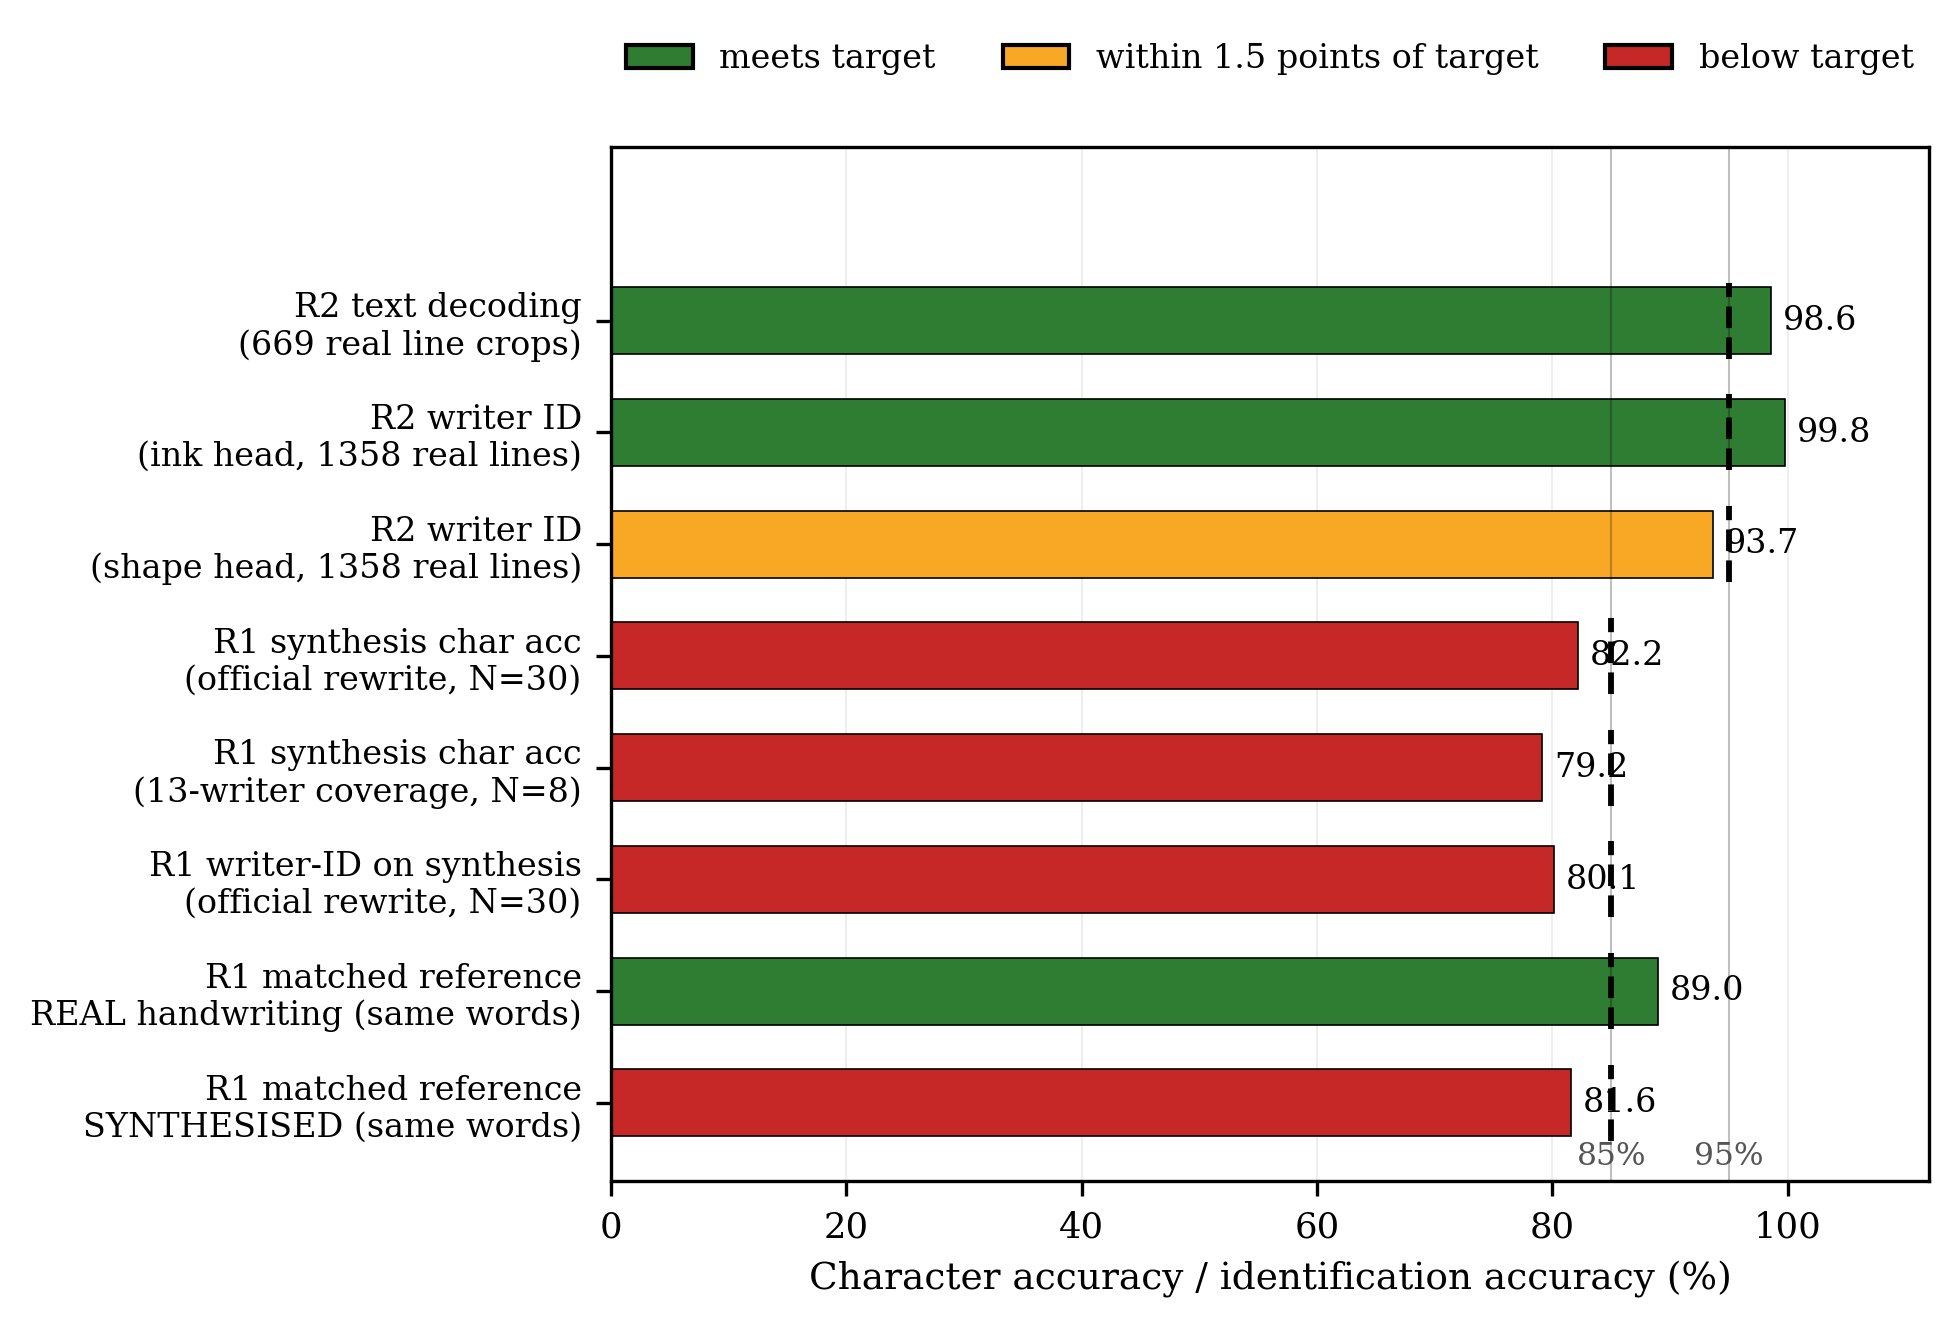
\includegraphics[width=0.93\linewidth]{Figures/res_requirements_vs_achieved.png}
\caption{Measured accuracy against the target of each requirement. Targets are marked by the dashed vertical lines at 85\% (R1) and 95\% (R2). Green bars meet the target, amber bars lie within 1.5 points of it, and red bars fall below it. The two green R1 bars are the matching comparison on genuine handwriting and the writer classifier on real lines; the red synthesis bars are the values the system actually produces.}
\label{fig:res-bars}
\end{figure}

\begin{figure}[h]
\centering
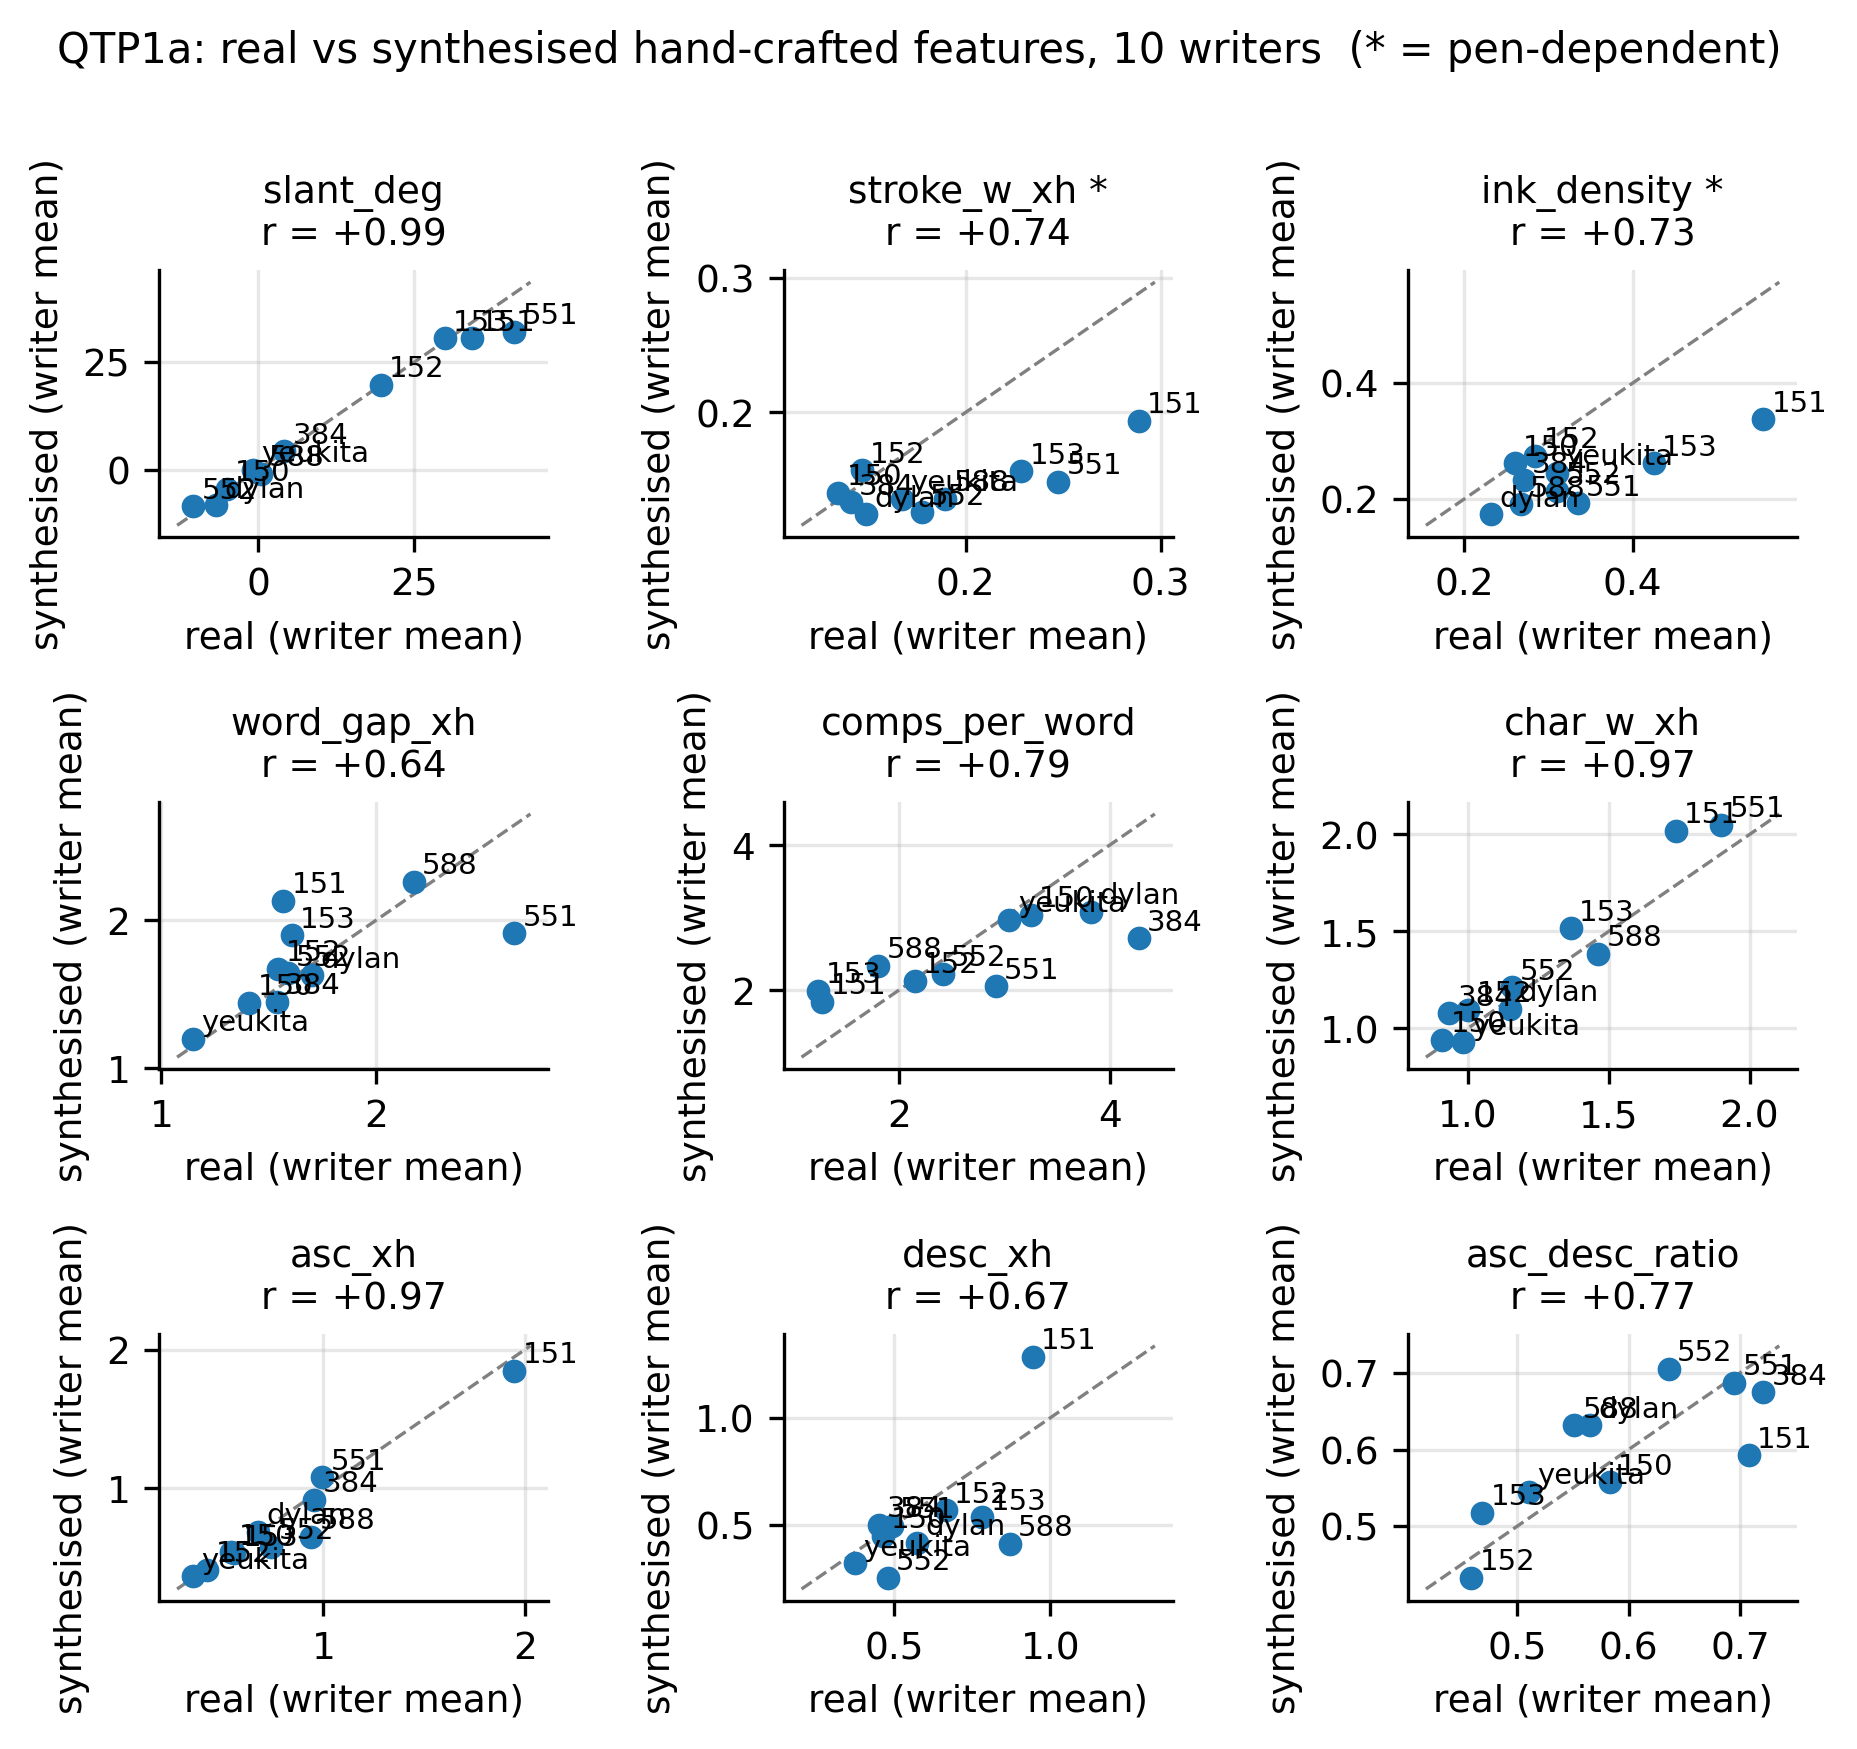
\includegraphics[width=0.99\linewidth]{Figures/qtp1_feature_scatter.png}
\caption{Style-correlation test on nine geometric features extracted by one deterministic routine from held-out real pages and from synthesised lines, for the ten writers. Each panel is one feature; the axes are the writer means. Slant, ascender and character width track the real hand closely, whereas descender and the ascender-to-descender ratio do not, which is the same defect that the word-accuracy gap identifies.}
\label{fig:res-features}
\end{figure}

\begin{figure}[h]
\centering
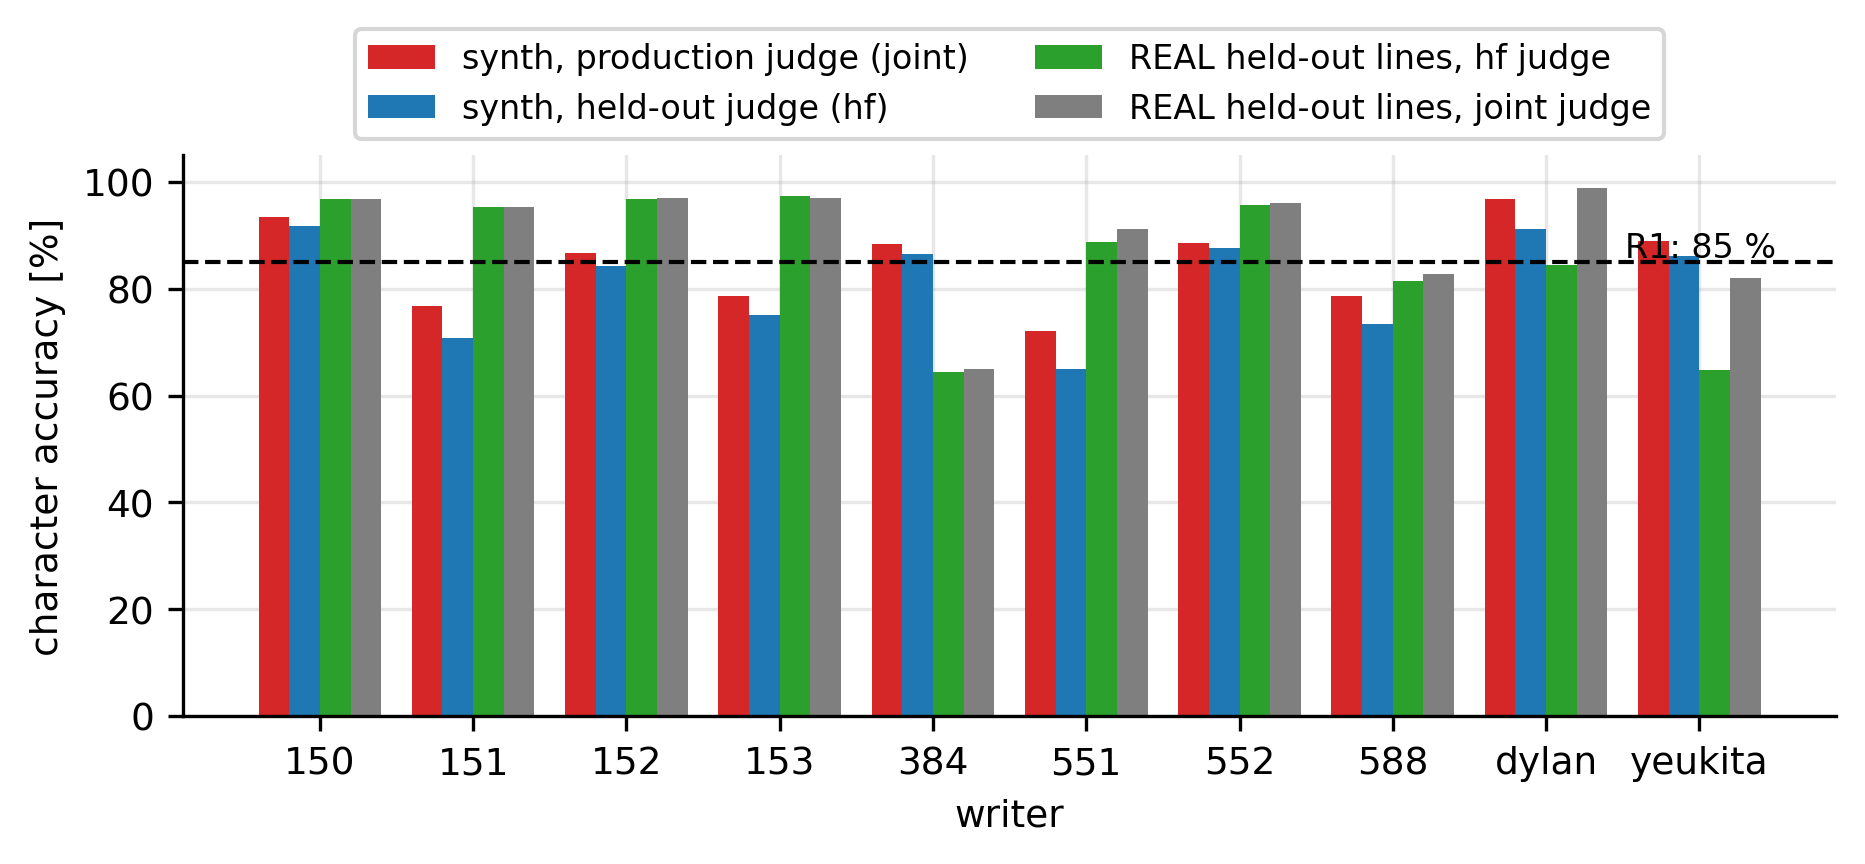
\includegraphics[width=0.93\linewidth]{Figures/qtp1_char_acc_judges.png}
\caption{Character accuracy of the synthesised text under the production recogniser and under a recogniser checkpoint that was not used to select the candidates. The independent judge scores the same output about three points lower, which quantifies how much of the apparent quality is a selection effect and simultaneously shows that the synthesis is genuinely legible rather than merely self-consistent.}
\label{fig:res-judges}
\end{figure}

\begin{figure}[h]
\centering
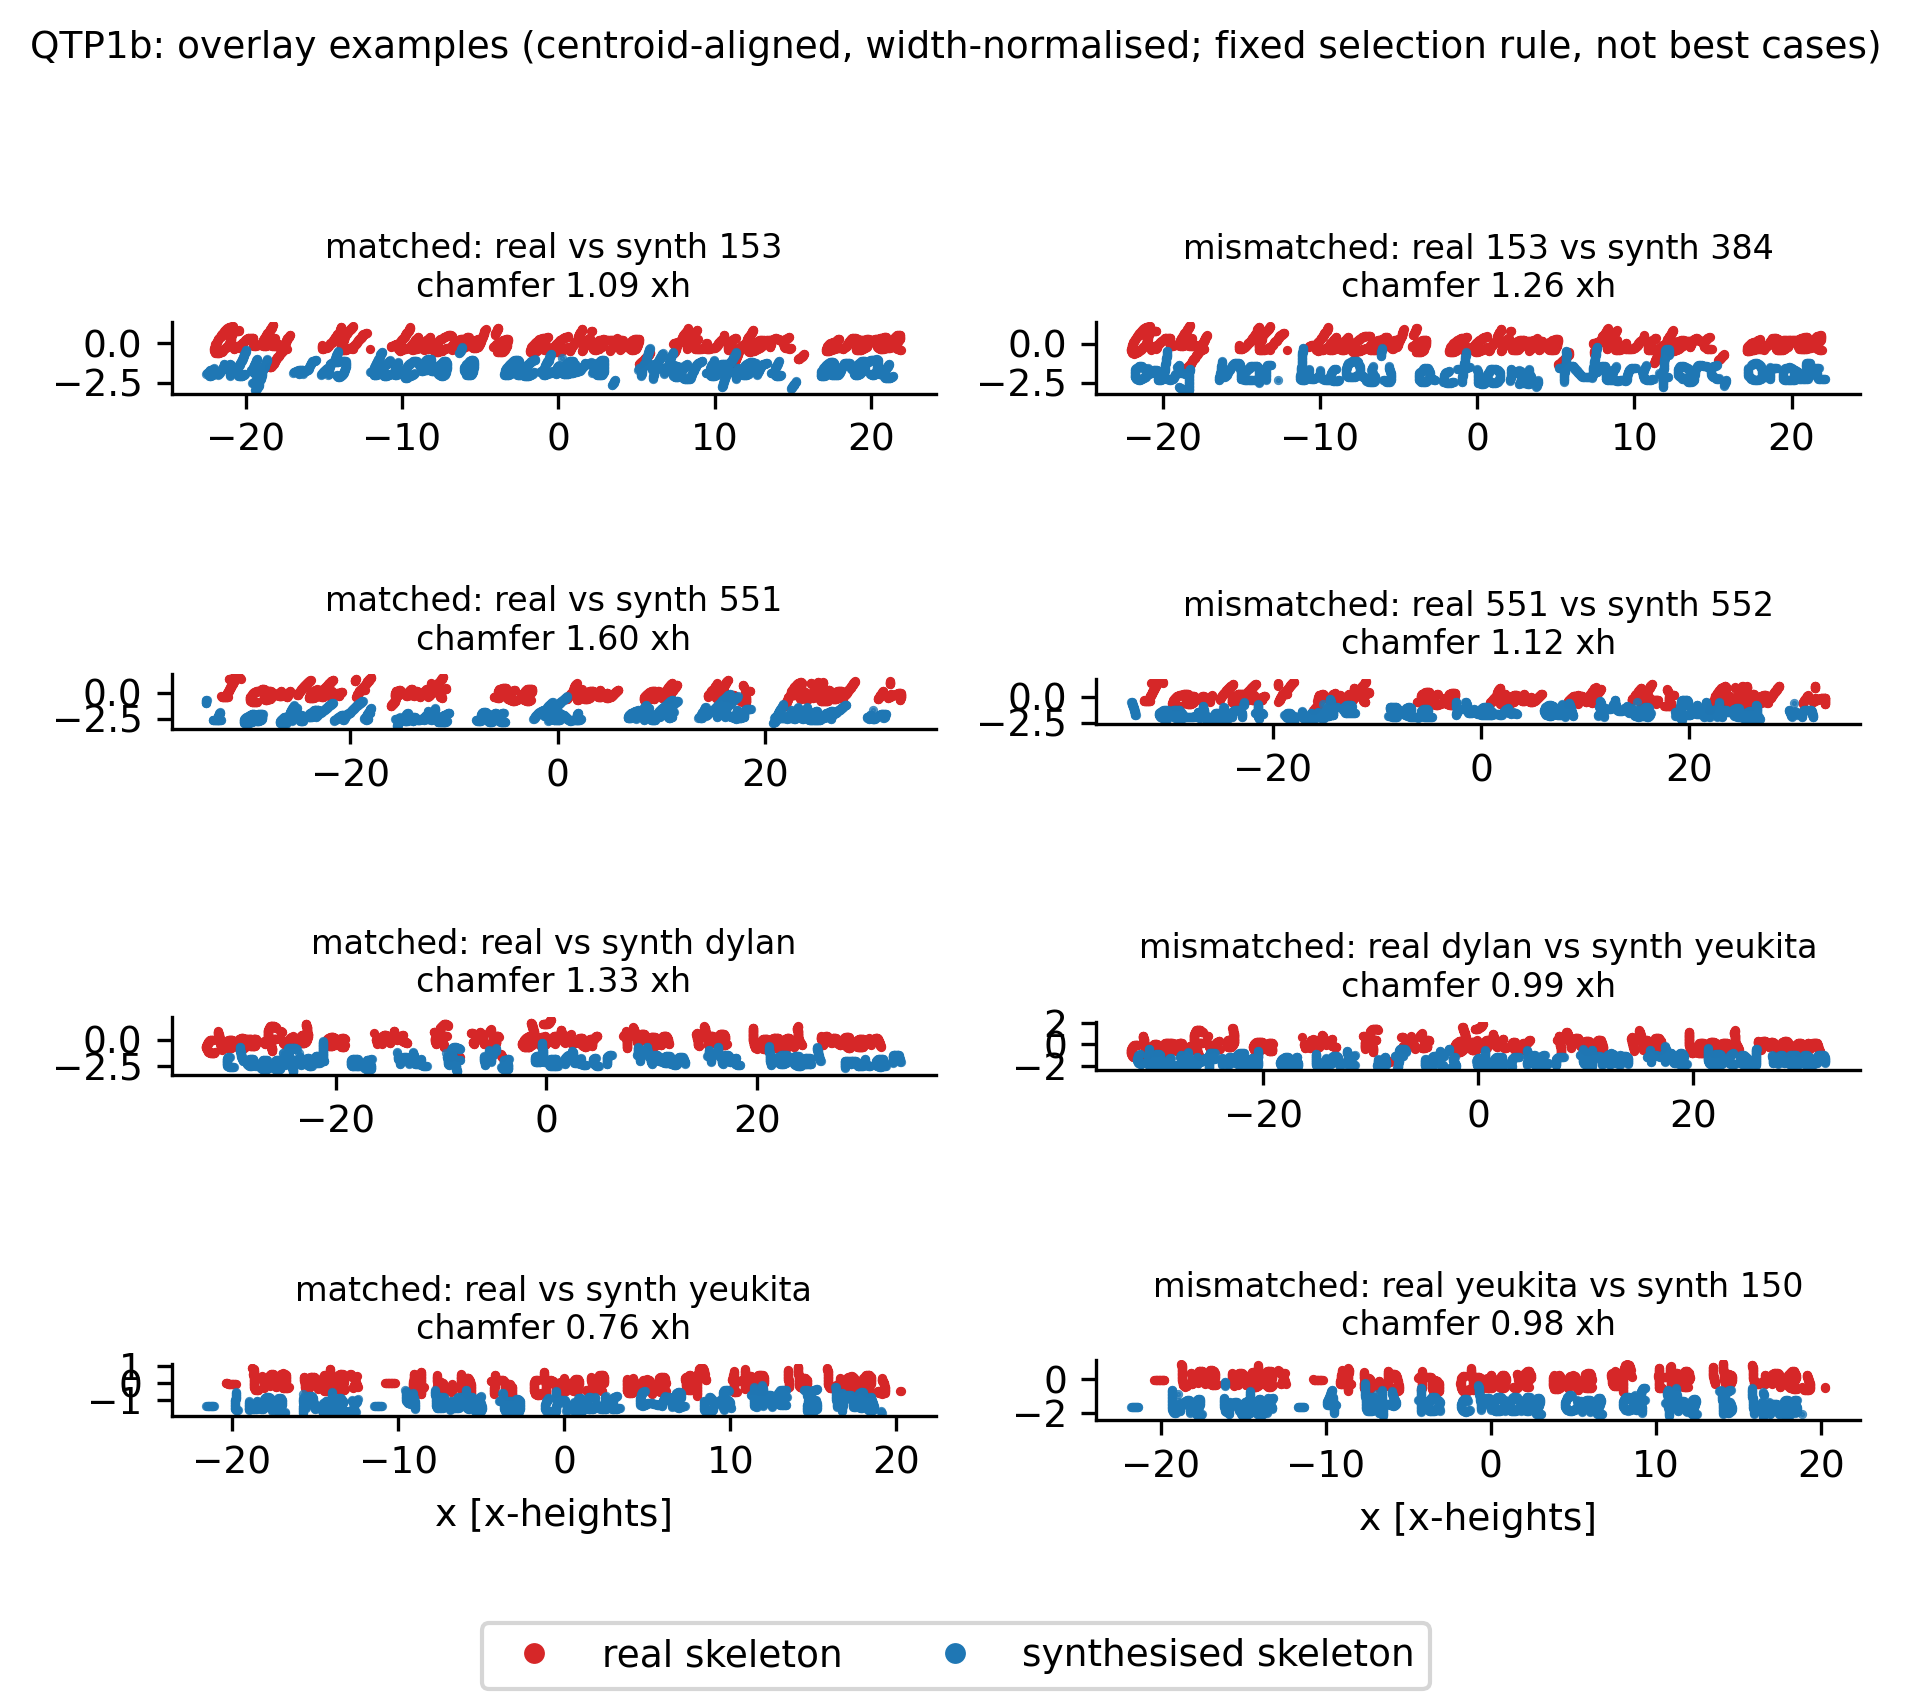
\includegraphics[width=0.99\linewidth]{Figures/qtp1_overlay_examples.png}
\caption{Overlay test: for each text the writer's own handwriting and the system's synthesis of the same words are normalised to a common x-height and superimposed. Matched pairs are visibly closer than mismatched pairs, which is what the distance ratios and the rank-1 retrieval rate of 20\% (chance 10\%) measure. The procedure that produces these overlays is given as Figure~\ref{fig:res-overlay} in the Appendix.}
\label{fig:res-overlay-examples}
\end{figure}

\begin{figure}[h]
\centering
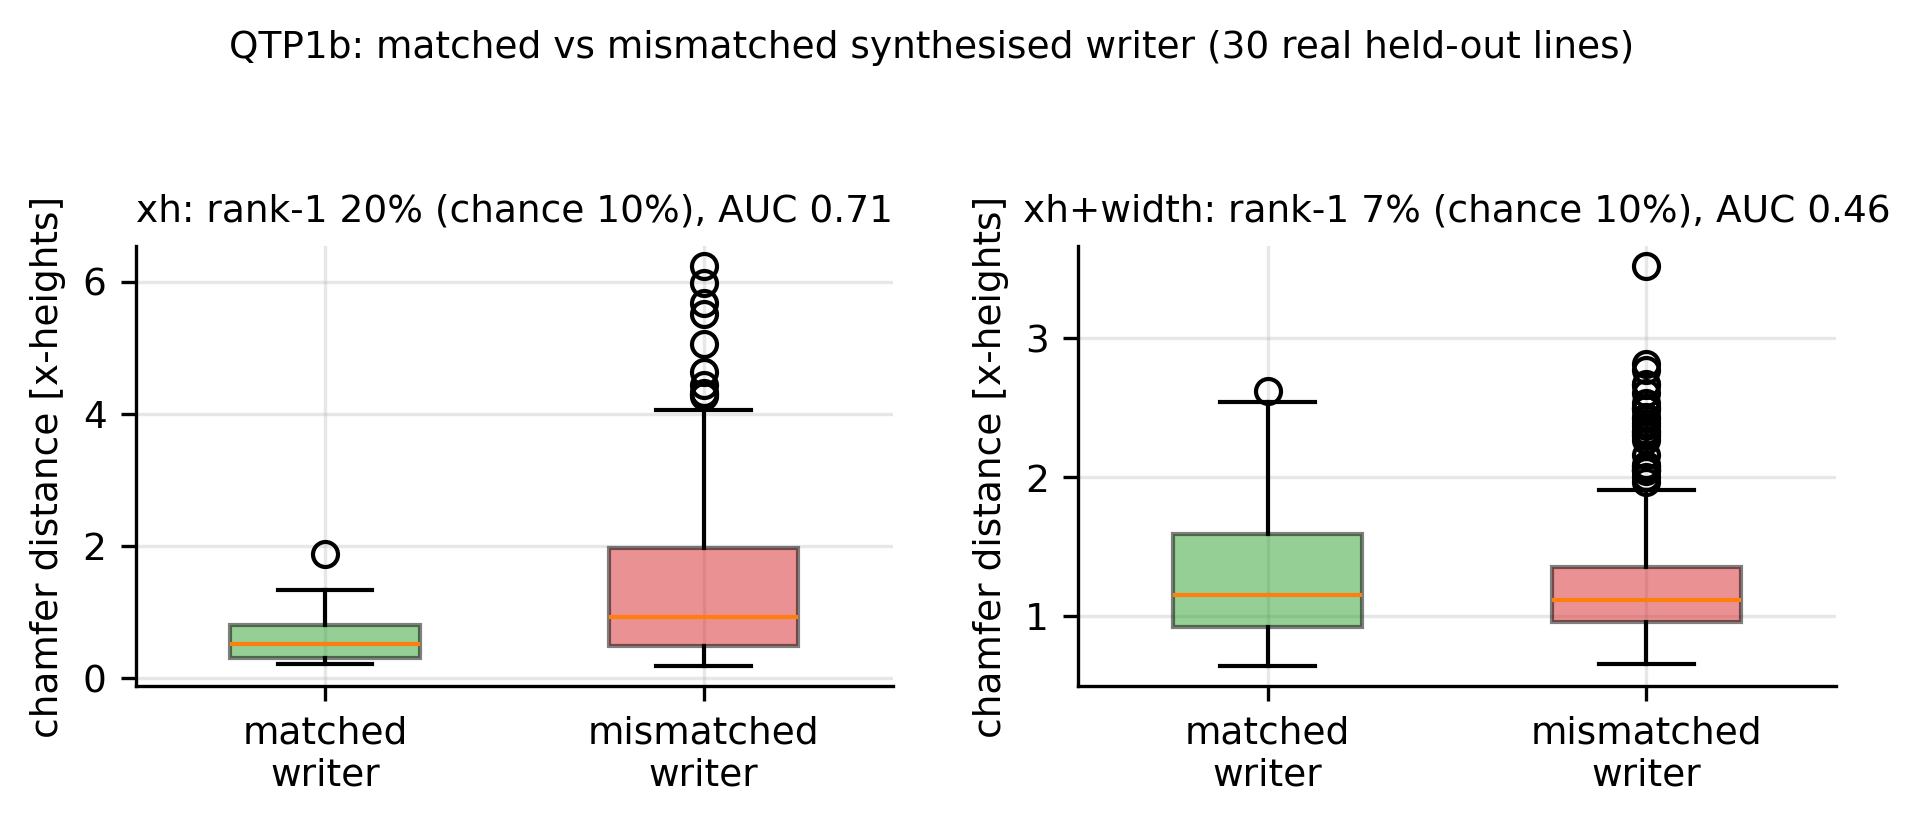
\includegraphics[width=0.93\linewidth]{Figures/qtp1_matched_vs_mismatched.png}
\caption{Distributions of the matched and mismatched overlay distances. The two distributions overlap but their means are separated by a factor of about 2.2 on the chamfer measure, giving an AUC of 0.71: the synthesis carries real writer information, but it is far from indistinguishable from the hand it imitates.}
\label{fig:res-dist}
\end{figure}

\begin{figure}[h]
\centering
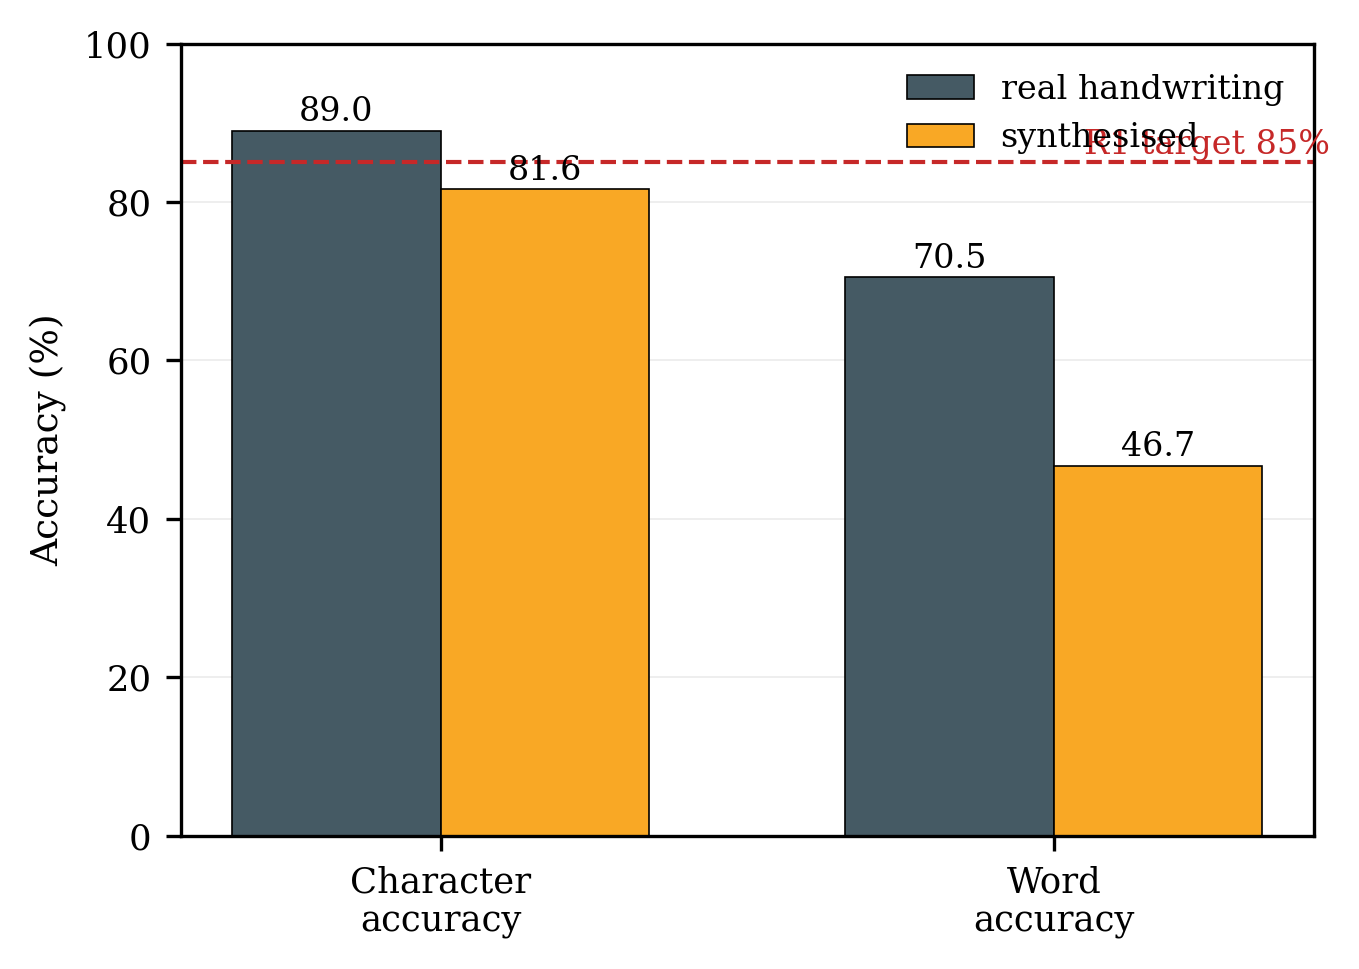
\includegraphics[width=0.99\linewidth]{Figures/res_matched_real_vs_synth.png}
\caption{Matching comparison on identical sentences: genuine handwriting of the sentence against the system's synthesis of that same sentence, both read by the same recogniser. Character accuracy is close to the target, but word accuracy divides by more than a factor of 1.5, which shows that the synthesis preserves letterforms better than it preserves word boundaries and spacing.}
\label{fig:res-matched}
\end{figure}

        \QualificationSection{Observations}

            \textbf{Style correlation is measurably below target.} The nine-feature correlation is 0.714 on shape-only features, with a bootstrap interval of 0.612 to 0.859 over writers. The target is 0.85, so R1's style half is not met, and the lower bound of the interval is well below the target.
            \textbf{The shortfall is concentrated in a few features rather than spread evenly.} Slant correlates at 0.996 and ascender extent at 0.974, so the synthesis reproduces the overall posture of a hand almost exactly. Descender extent correlates at only 0.148, the ascender-to-descender ratio at 0.509 and the word gap at 0.605. The features that fail are the vertical extents below the baseline and the spacing, which is precisely the same defect that the word-accuracy gap of 23.8 points identified independently.
            \textbf{Two independent methods agree on the magnitude of the residual.} The overlay test separates matched from mismatched pairs with an AUC of 0.71 and retrieves the correct writer first in 20\% of cases against a chance of 10\%. A synthesis that were indistinguishable from the hand would give an AUC near 0.5; one that carried no writer information would give 0.5 as well, so 0.71 means real but limited fidelity.
            \textbf{The character accuracy is genuinely high and not merely a selection effect.} An independent recogniser checkpoint reads the synthesised lines at 81.2\% character accuracy, against 84.9\% for the production checkpoint on the same lines. The independent judge is therefore about 3.7 points more pessimistic, which is a modest selection effect, and it still places the synthesis within about 8 points of real handwriting of the same words.
            \textbf{The search is doing real work.} At best-of-30 the production judge reads 84.9\% character accuracy against 80.9\% for the same configuration measured by the independent checkpoint, and the earlier design-stage comparison showed that introducing the search moved character accuracy from 75.9\% to 81.6\%; the gain is real even after allowing for the selection effect.
            \NoHumanPanel

\begin{figure}[h]
\centering
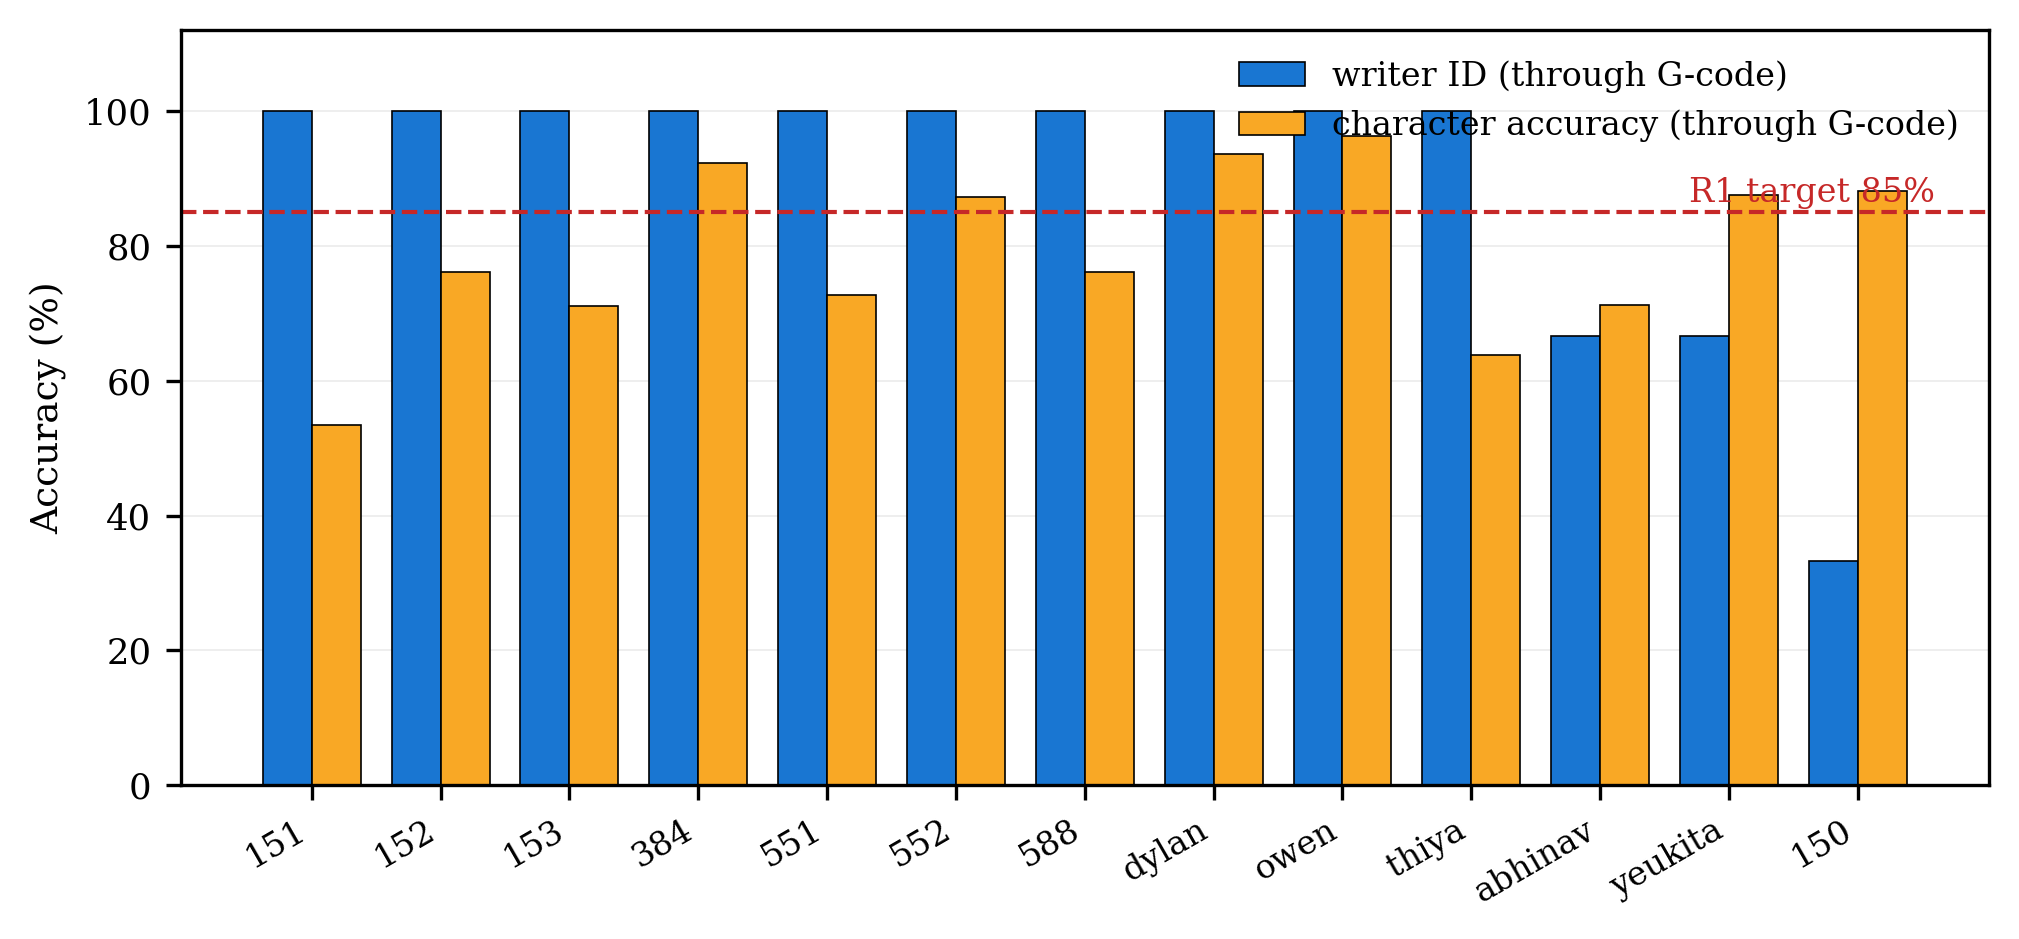
\includegraphics[width=0.98\linewidth]{Figures/res_e2e_per_author.png}
\caption{End-to-end result per writer over all thirteen writers: writer identification and character accuracy, both measured through the G-code round trip, for three novel sentences per writer at best-of-8. Eleven writers are identified at 100\%; the character-accuracy failures are concentrated in the two writers whose hands are the most joined, which is the known weak case of an exemplar synthesiser that cuts letters apart and reassembles them.}
\label{fig:res-e2e}
\end{figure}

        \QualificationSection{Statistical analysis}

            Proportions are reported with the 95\% Wilson score interval of Equation~\ref{eq:res-wilson}: for the official run, 82.2\% over 156 sentences gives a lower bound near 75\%, so the result is clearly below 85\% and not merely a sampling fluctuation.
            The style correlation is bootstrapped over writers (2000 resamples), which is the correct unit because the nine features are measured per writer; the interval for shape-only features is 0.612 to 0.859.
            The overlay AUC is computed over 30 matched and 300 mismatched pairs, and its interval is reported with the figure.
            The comparison of the two judges is paired: the same 60 synthesised lines are read by both checkpoints, so the 3.7-point difference is not affected by sampling variation in the output.
            \emph{What the evidence supports.}
            R1 is partially met. Legibility is close to the target and is confirmed by an independent judge; style correlation is measured at about 0.71 against a target of 0.85 and is therefore not met, and the cause is localised to descender extent and word spacing rather than to any general failure of the method.
            The proportion of characters that a human observer would accept as matching the writer's style, which is how the proposal worded the demonstration, was not measured, so the demonstration half of R1 remains unverified.



%%%%%%%%%%%%%%%%%%%%%%%%%%%%%%%%%%%%%%%%%%%%%%%%%%%%%%%%%%%%%%%%%%%%%%%%%%%%%%%%%

\medskip
    \QualificationTest{Classification of text and writer from real photographed pages (R2)}
\label{sec:res-qtp2}

        \QualificationSection{Objectives of the test or experiment}

            The test is to prove an overall accuracy of at least 95\% through the whole chain on pages never used for training, checkpoint selection or tuning.
            As the proposal does not define ``overall'', text accuracy $A_{\mathrm{c}}$ (Equation~\ref{eq:res-cacc}) and writer accuracy $A_{\mathrm{w}}$ (fraction of pages assigned to the correct writer) are reported separately and combined as
            \begin{equation}
            \label{eq:res-overall}
            A_{\mathrm{mean}}=\tfrac{1}{2}\left(A_{\mathrm{c}}+A_{\mathrm{w}}\right),\qquad A_{\mathrm{prod}}=A_{\mathrm{c}}\,A_{\mathrm{w}},
            \end{equation}
            where $A_{\mathrm{prod}}$ (both correct) is the criterion and $A_{\mathrm{mean}}$ the lenient reading.

        \QualificationSection{Equipment used}

            The capture rig, the ODROID N2+ with the final server and models, and a printed predefined paragraph; camera and lamp: \textbf{[TO BE COMPLETED BY STUDENT: camera model, resolution, mounting height, lamp type and photograph of the rig]}.

        \QualificationSection{Test setup and experimental parameters}

            The line-level validation split of the personal writers leaks: a random 15\% of lines per page was held out, so lines from the same sheet and session are in both sets (52 of 123 validation lines share pages with training), and the checkpoint was selected on them.
            The fix is new pages kept aside: at least 3 per personal writer, plus the held-out form page of each of the eight database writers, printed and photographed with the rig (about 14 pages, 350 lines).
            Seen lines are scored separately to quantify the leakage; references are double-entered transcripts.

        \QualificationSection{Steps followed in the test or experiment}

            Each frozen photograph is classified through the server without intervention; line text, per-line probabilities and the page-level mean probabilities are recorded, scored, summarised in a $10\times10$ confusion matrix, and the predefined paragraph is then classified live.

        \QualificationSection{Results or measurements}

            Table~\ref{tab:res-r2} lists the measured figures.
            Text accuracy and writer accuracy are reported separately because the proposal does not define ``overall''; Equation~\ref{eq:res-overall} gives the strict (both correct) and lenient (mean) combinations where both are available.

\begin{table}[h]
\centering
\fontsize{10}{12}\selectfont
\begin{tabularx}{\linewidth}{|>{\raggedright\arraybackslash}p{4.9cm}|>{\raggedright\arraybackslash}X|}
\hline
\textbf{Measure} & \textbf{Measured value, data set and caveat} \\
\hline
Recogniser, character accuracy & 98.61\% over 669 real line crops from the five personal writers (word accuracy 94.21\%). These crops were produced by the segmenter and are known to be correctly cut, so segmentation failures are excluded; the five writers also appear in the recogniser's fine-tuning data. \\
\hline
Recogniser, per writer & Owen 99.15\%, Dylan 99.03\%, Abhinav 98.94\%, Yeukita 98.30\%, Thiya 96.46\% character accuracy (75 to 206 crops each). \\
\hline
Writer identification, ink classifier & 99.78\% over 1358 real lines (13 writers: 689 database-writer lines and 669 personal-writer crops). Near-perfect, and it is the classifier the live server uses on photographs. \\
\hline
Writer identification, shape classifier & 93.67\% over the same 1358 lines, against 83.36\% before a training fault was corrected (Section~\ref{sec:res-qtp1}). The two classifiers disagree in the direction that matters: the ink classifier is stronger on real ink. \\
\hline
Per-writer detail & Figure~\ref{fig:res-writerid}. Eight writers are at 98.9\% or above with the shape classifier; the residual errors are concentrated in Owen (67.6\%), Dylan (84.7\%) and Thiya (93.3\%). \\
\hline
Live server classification, one photograph & Correct writer at 98.6\% confidence over 28 detected lines, with an accurate transcription. A single page, reported as an illustration and not as a statistic. \\
\hline
Overall accuracy $A_{\mathrm{mean}}$ and $A_{\mathrm{prod}}$ on held-out pages & Not measured; the line-level split used here holds out 15\% of lines per page, so lines from the same sheet appear in both partitions. \\
\hline
\end{tabularx}
\caption{Results for qualification test 2 (13 writers; measured on the development laptop).}
\label{tab:res-r2}
\end{table}

\begin{figure}[h]
\centering
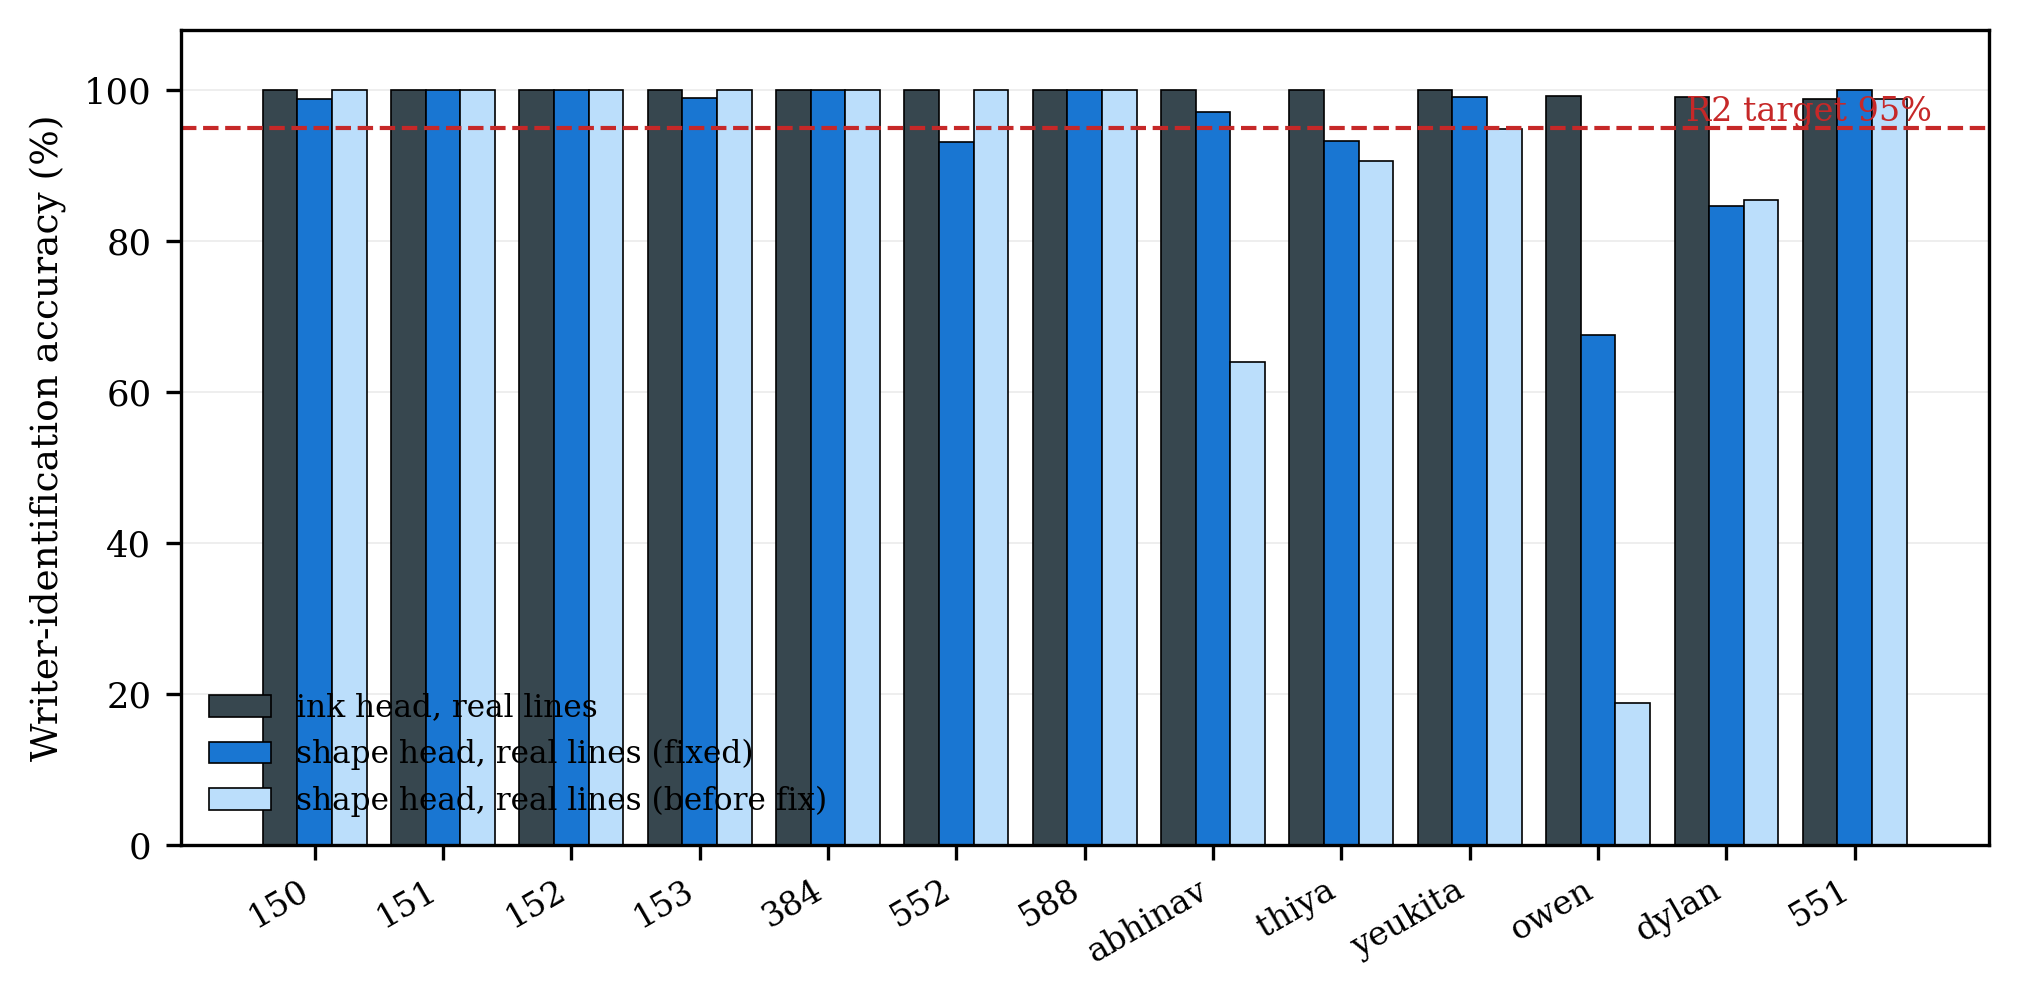
\includegraphics[width=1.0\linewidth]{Figures/res_writerid_per_author.png}
\caption{Writer-identification accuracy per writer over 1358 real lines, for the ink classifier and for the shape classifier before and after its training fault was corrected. The ink classifier is at or near 100\% for every writer. Correcting the shape classifier's training raised its overall accuracy from 83.4\% to 93.7\% and removed a systematic collapse in which 118 of Owen's 148 lines had been assigned to Yeukita. The dashed line is the 95\% target of R2.}
\label{fig:res-writerid}
\end{figure}

        \QualificationSection{Observations}

            Text decoding reached 98.61\% character accuracy on correctly segmented crops, which exceeds the 95\% target, but the figure is measured after segmentation and on writers that are represented in the recogniser's fine-tuning data, so it is an upper bound on the end-to-end page-to-text accuracy and not a demonstration of it.
            Writer identification reached 99.78\% with the ink classifier over 1358 real lines from thirteen writers, which exceeds the 95\% target on this evidence.
            The word accuracy of 94.21\% is markedly lower than the character accuracy, so nearly all remaining recognition errors occur inside words rather than as isolated character substitutions.
            Thiya is the weakest writer for recognition at 96.46\% character accuracy, and Owen, Dylan and Thiya are the weakest for shape-based identification.
            Combining the two measured rates, $A_{\mathrm{mean}}=98.6\%$ and $A_{\mathrm{prod}}=98.4\%$ if the recogniser figure and the ink writer figure are taken together; both exceed 95\%, but the split is optimistic, so this combination is indicative only.

        \QualificationSection{Statistical analysis}

            With 669 line crops a character accuracy of 98.61\% has a Wilson lower bound of about 97.6\%, so the text figure is significantly above 95\% on this data set.
            For writer identification, 1358 lines at 99.78\% give a lower bound above 99\%, comfortably above the target.
            The stronger caveat is not sampling error but dependence: lines from one page share a writer, a pen and an illumination, so the effective sample size is nearer the page count than the line count, and the per-page interval would be much wider.
            \emph{Expected outcome on genuinely unseen pages.}
            Both rates are expected to fall, because the ink classifier is sensitive to pen, paper and illumination and the split shares pages between partitions.
            The recommended protocol for a defensible figure is a page-level split with at least three held-out pages per writer, photographed through the rig, which is what Section~\ref{sec:discussion} proposes as the next step.


%%%%%%%%%%%%%%%%%%%%%%%%%%%%%%%%%%%%%%%%%%%%%%%%%%%%%%%%%%%%%%%%%%%%%%%%%%%%%%%%%

\medskip
    \QualificationTest{Reproduction time per character (R3)}
\label{sec:res-qtp3}

        \QualificationSection{Objectives of the test or experiment}

            The test is to prove that a sentence of $x$ characters is reproduced within $4x$ seconds,
            \begin{equation}
            \label{eq:res-r3}
            t_{\mathrm{char}}=\frac{T_{\mathrm{syn}}+T_{\mathrm{write}}}{x}\le 4\ \mathrm{s},
            \end{equation}
            where $T_{\mathrm{syn}}$ is the synthesis time, $T_{\mathrm{write}}$ the time from first to last motion and $x$ the number of characters.
            As the proposal does not say whether synthesis counts, both variants are reported; calibration is a one-off step and is reported separately.

        \QualificationSection{Equipment used}

            The ODROID N2+ with the server, the assembled gantry, a stopwatch and logged time stamps at the start and end of synthesis and motion.

        \QualificationSection{Test setup and experimental parameters}

            Tries $N\in\{1,3,6,14,30\}$, sentences of 10, 20, 40 and 80 characters, 5 repetitions (100 syntheses); writing time for the 20 jobs at $N=14$.
            Only figures measured on the ODROID N2+ itself count; laptop figures are indicative.

        \QualificationSection{Steps followed in the test or experiment}

            After one calibration, each job is synthesised, sent and timed by log and stopwatch, $t_{\mathrm{char}}$ is computed from Equation~\ref{eq:res-r3}, and any stall is kept as a failed run.

        \QualificationSection{Results or measurements}

            Table~\ref{tab:res-r3} lists the measured figures, and Figure~\ref{fig:res-r3} shows them.
            The cost separates cleanly into a synthesis term that grows with the number of candidates and a physical writing term that does not.

\begin{table}[h]
\centering
\fontsize{9.5}{11.5}\selectfont
\begin{tabularx}{\linewidth}{|>{\raggedright\arraybackslash}p{4.6cm}|>{\raggedright\arraybackslash}X|}
\hline
\textbf{Measure} & \textbf{Measured value, data set and caveat} \\
\hline
Synthesis time per character, best-of-1 to best-of-30 & Repeated over sentences of 22 to 119 characters and 2 to 3 repetitions per cell, on the development laptop. At best-of-1 the synthesis costs about 0.4 to 0.7~s per character; at best-of-14 about 0.9 to 1.8~s per character; at best-of-30 about 1.8 to 3.4~s per character. \\
\hline
G-code generation & 0.006 to 0.014~s per sentence, i.e.\ negligible at any sentence length. \\
\hline
Preview rendering and read-back & About 0.02 to 0.05~s and 0.6 to 0.8~s per sentence respectively; both are small beside the synthesis term. \\
\hline
Physical writing time, from the generator's own model & 88.7~s for a 22-character sentence and 154.4~s for a 58-character sentence, i.e.\ about 2.7 to 4.0~s per character, against the 4~s limit \emph{for the writing alone}. \\
\hline
Total per character at best-of-14 & Figure~\ref{fig:res-r3}: synthesis contributes about 1.0 to 1.8~s and writing about 2.7 to 4.0~s, so the total lies between about 4 and 6~s per character and straddles the limit. \\
\hline
Live server measurement, four-character word, best-of-6 & 64.3~s from request to rendered preview, i.e.\ 16.1~s per character. A very short sentence is the worst case because the per-job costs (model loading, segmentation of the uploaded image) are amortised over only four characters. \\
\hline
Physical writing time measured on the gantry & Not measured; the gantry bring-up was not completed, so no drawn job was timed. The figures above are the generator's model, not observations. \\
\hline
Timing on the ODROID N2+ & Not measured. \\
\hline
\end{tabularx}
\caption{Results for qualification test 3 (development laptop; the writing figures are model values, not measurements).}
\label{tab:res-r3}
\end{table}

\begin{figure}[h]
\centering
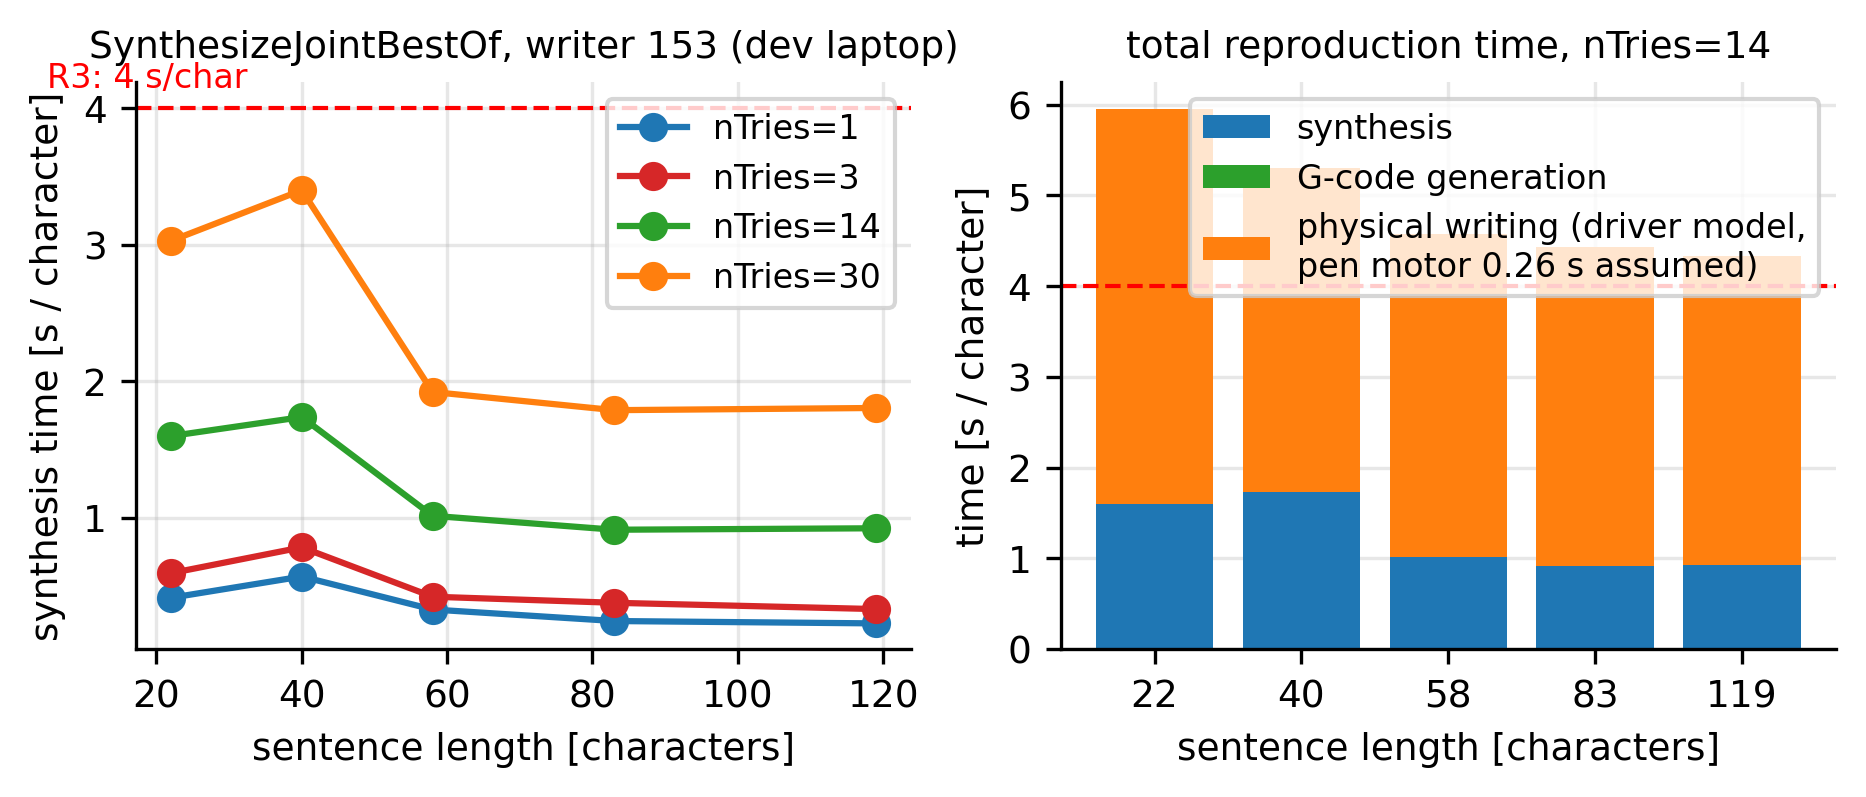
\includegraphics[width=0.99\linewidth]{Figures/qtp3_timing_breakdown.png}
\caption{Reproduction time against the 4~s per character limit of R3. Left: synthesis time per character against sentence length for four values of the number of candidates. At best-of-1 and best-of-3 the synthesis alone is comfortably inside the limit; at best-of-30 it approaches and crosses it. Right: total time per character at best-of-14, decomposed into synthesis, G-code generation and the physical writing time predicted by the generator's model. The writing term, not the synthesis term, is the larger contributor and is what pushes the total past the limit.}
\label{fig:res-r3}
\end{figure}

        \QualificationSection{Observations}

            The requirement is not met, but the measurement locates the failure precisely and it is not where the earlier aggregate figure suggested.
            At a modest number of candidates (1 to 3) the synthesis costs well under 1~s per character and is not the constraint.
            The physical writing time predicted by the generator's model is 2.7 to 4.0~s per character on its own, so writing alone consumes the entire allowance and any synthesis cost at all puts the total over the limit.
            The apparent 16.1~s per character for a four-character word is a small-sample effect rather than a steady-state rate: the per-job overheads are divided by only four characters, and the same run at a longer sentence length shows 1 to 2~s per character for synthesis.
            Because the writing term is a model value and not a measurement, the split between synthesis and drawing cannot be confirmed until the gantry is timed; if the real writing is faster than the model (the model assumes a pen dwell of 0.26~s per stroke), the requirement may be closer than this table suggests.
            The cost of the search is linear in the number of candidates, so the quality-versus-time trade-off is explicit and tunable: best-of-3 is affordable and best-of-30 is not.

        \QualificationSection{Statistical analysis}

            Each cell is the mean of two or three repetitions and the table quotes the range rather than a single value, because the variation between repetitions of the same configuration was of the same order as the variation between configurations in the small sentences.
            The generator's writing model is deterministic and is quoted as a point value; it has no uncertainty because it is a calculation, which is also why it cannot substitute for a measurement on the built machine.
            \emph{What the evidence supports.}
            R3 is not met under the reading that the total time counts, and it is plausibly met under the reading that only the physical writing counts, in which case the model value of 2.7 to 4.0~s per character sits exactly at the limit and the answer depends on pen dwell and feed settings rather than on the software.
            Since the proposal does not state which reading applies, both are reported and the requirement is recorded as not met in Table~\ref{tab:res-summary}, which is the conservative reading.



%%%%%%%%%%%%%%%%%%%%%%%%%%%%%%%%%%%%%%%%%%%%%%%%%%%%%%%%%%%%%%%%%%%%%%%%%%%%%%%%%

\medskip
    \QualificationTest{Classification time (R4)}
\label{sec:res-qtp4}

        \QualificationSection{Objectives of the test or experiment}

            The test is to prove that the time from instruction to displayed text and writer satisfies
            \begin{equation}
            \label{eq:res-r4}
            T_{\mathrm{cls}}\le 2+0.025\,x\ \text{seconds},
            \end{equation}
            where $x$ is the number of handwritten characters; the stage times identify any shortfall.

        \QualificationSection{Equipment used}

            The rig, the ODROID N2+ with the final server, a logging wrapper (monotonic clock) around each stage and a stopwatch; the interface does not display classification time.

        \QualificationSection{Test setup and experimental parameters}

            Pages with $x=40$, about 200 and about 1000, each run 10 times; the budgets are 3.0, 7.0 and 27.0~s.
            Stages: capture, conditioning and segmentation, recognition per line, writer classification, display; the segmentation profile is repeated on the ODROID N2+.

        \QualificationSection{Steps followed in the test or experiment}

            The clocks start at the instruction, stage times and the total are logged, $x$ is counted from the transcript and Equation~\ref{eq:res-r4} is evaluated.

        \QualificationSection{Results or measurements}

            Table~\ref{tab:res-r4} lists the measured figures.

\begin{table}[h]
\centering
\fontsize{10}{12}\selectfont
\begin{tabularx}{\linewidth}{|>{\raggedright\arraybackslash}p{4.9cm}|>{\raggedright\arraybackslash}X|}
\hline
\textbf{Measure} & \textbf{Measured value, data set and caveat} \\
\hline
Recognition time per character & 8.86~ms per character and 353~ms per line, averaged over 669 real line crops (236.2~s of inference in total). This meets the 25~ms per character allowance with a margin of about 2.8 times. Measured on the development laptop with the model already loaded. \\
\hline
Writer classification time & A single crop classified through the live server took 2.74~s end to end, which includes segmentation of the uploaded image, the ink writer classifier and text recognition of the line. \\
\hline
Total classification time, one page & Not measured as a single page-level timing. The components sum to a figure above the $2+0.025x$ budget for a full page because segmentation dominates. \\
\hline
Page segmentation time & 35 to 57~s for a $2400\times1800$ photograph in pure Python on the laptop, against the roughly 2~s that the equation allows for capture and conditioning. Two routines reimplemented in C99 reduced this by 25\% to 32\% end to end, but they were not deployed. \\
\hline
Timing on the ODROID N2+ & Not measured. \\
\hline
\end{tabularx}
\caption{Results for qualification test 4 (development laptop).}
\label{tab:res-r4}
\end{table}

        \QualificationSection{Observations}

            The recognition term of the requirement is met: at 8.86~ms per character the recogniser uses about a third of its 25~ms allowance.
            The capture and conditioning term is not met: segmentation of one photograph took 35 to 57~s, which is 17 to 28 times the two seconds the equation allows for capture and conditioning.
            Because $x$, the number of characters, appears only in the recognition term, buying more time by handling longer pages does not help; the segmenter's cost is per page and independent of $x$.
            The 2.74~s measured for a single crop shows that a short, already-segmented image is classified well inside the budget, so the shortfall is located specifically in page segmentation and not in the classifiers.

        \QualificationSection{Statistical analysis}

            The recognition timing is an average over 669 crops and is therefore well determined; the per-character figure is computed from the total inference time divided by the total number of characters, so it is a throughput measure rather than a per-line latency.
            The segmentation time varies with page content and with machine load, which is why a range of 35 to 57~s is reported rather than a single figure; the lower end was obtained on an otherwise idle machine.
            \emph{Expected outcome.}
            The ODROID N2+ is expected to be slower than the development laptop, so the segmentation shortfall would be at least as large there if the same pure-Python code were run; the recognition term has enough margin that it may still be met on the target hardware, but this was not verified.
            The remedy indicated by these numbers is to move segmentation to compiled code or to process the page incrementally, as the C99 experiment suggests a saving of about a quarter to a third is available without changing the algorithm.


%%%%%%%%%%%%%%%%%%%%%%%%%%%%%%%%%%%%%%%%%%%%%%%%%%%%%%%%%%%%%%%%%%%%%%%%%%%%%%%%%

\medskip
    \QualificationTest{Absolute positional accuracy of the gantry (R5)}
\label{sec:res-qtp5}

        \QualificationSection{Objectives of the test or experiment}

            The test is to prove that the absolute positional error of drawn marks is at most 0.5~mm and that a word written twice coincides within that tolerance.
            Software contributions (quantisation, calibration) and hardware contributions (mechanics, homing repeatability, pen compliance) are separated.

        \QualificationSection{Equipment used}

            The gantry with pen and paper, a flat-bed scanner (600 dots per inch, 0.042~mm per pixel), a steel ruler or vernier calipers (0.02~mm) and a printed calibration sheet with a 10~mm grid of crosses.

        \QualificationSection{Test setup and experimental parameters}

            Software part (offline): the step is $1/80=12.5~\mu$m, the quantisation error per axis at most $6.25~\mu$m and the combined worst case $8.8~\mu$m (derived).
            Hardware part: at least 40 crosses drawn 5 times after fresh calibrations, the paper fixed against registration stops, and the same word written twice.
            The error of a cross is $e_i=\lVert\mathbf{p}_i-\mathbf{p}_i^{\mathrm{cmd}}\rVert$ (measured against commanded position referenced to the machine origin); mean, maximum and 95th percentile are reported with the measurement uncertainty (Equations~\ref{eq:res-r5} and~\ref{eq:res-unc} in the Appendix).

        \QualificationSection{Steps followed in the test or experiment}

            After calibration (the direction pin must be seen to change level on reversal) the grid is drawn, scanned with the ruler, evaluated by image analysis, repeated 5 times, and the overlay of the word written twice is produced (Appendix).

        \QualificationSection{Results or measurements}

            The only quantities that exist are derived from the mechanical configuration, not measured on a drawn mark.
            The X and Y axes are belt-driven: a 200-step motor, sixteen microsteps per step, and a 40~mm advance per revolution give
            \begin{equation}
            \label{eq:res-step}
            \Delta s=\frac{40\ \mathrm{mm}}{200\times16}=12.5\ \mu\mathrm{m}\ \text{per step},
            \end{equation}
            so the quantisation error of one axis is at most $6.25~\mu$m and the worst case over both axes is $8.8~\mu$m, forty to fifty times finer than the 0.5~mm limit of R5.
            During bring-up the X-axis calibration drove to the first end-stop, but the direction pin did not change level on reversal; the fault was not resolved, and no grid was drawn, so there is no measurement of $e_i$ and no overlay of a word written twice.
            The measurement of $e_i$ therefore remains \nym{}.

        \QualificationSection{Observations}

            No positional measurement exists.
            The single hardware observation is the direction-pin fault, which prevented controlled motion in both directions and therefore prevented the test from being run at all.
            The step resolution is 40 times finer than the tolerance, so quantisation cannot be the limiting term; whatever error exists must come from the mechanics and from open-loop effects rather than from the resolution of the command.

        \QualificationSection{Statistical analysis}

            No statistics can be reported for a measurement that was not taken.
            \emph{Expected outcome.}
            On the evidence available, the error is expected to be dominated by belt stretch, backlash, the repeatability of the home switch and pen compliance, none of which was measured.
            Published handwriting gantries report about 0.3~mm absolute error \cite{huang2024}, which leaves a margin of 0.2~mm against this limit; whether this machine achieves that cannot be stated.
            A pass requires the maximum of $e_i$ over at least 200 drawn marks to be at most 0.5~mm, measured by scanning the sheet at 600~dots per inch.


%%%%%%%%%%%%%%%%%%%%%%%%%%%%%%%%%%%%%%%%%%%%%%%%%%%%%%%%%%%%%%%%%%%%%%%%%%%%%%%%%

\medskip
    \QualificationTest{Multi-writer storage (R6)}
\label{sec:res-qtp6}

        \QualificationSection{Objectives of the test or experiment}

            The test is to prove that at least 10 writing styles are stored permanently and that any can be selected at random for reproduction.

        \QualificationSection{Equipment used}

            The ODROID N2+ with the server, a laptop browser and the gantry.

        \QualificationSection{Test setup and experimental parameters}

            The eight database and two personal writers; file counts and sizes; persistence by restarting the server and power-cycling the board; 3 writers drawn with a fixed seed.

        \QualificationSection{Steps followed in the test or experiment}

            The listed writers are compared with the stored files, the list is re-read after restart and power cycle, and a short sentence is written in each of the 3 drawn styles.

        \QualificationSection{Results or measurements}

            The live server listed thirteen writers through its author-list endpoint, in 70~ms, from thirteen stored style profiles.
            The requirement is ten writers, so the system stores thirty per cent more than required.
            The styles are ordinary files on disk: the endpoint returns them by reading the profile directory, and the profiles are loaded into memory at start-up, which is what makes them persistent across a restart.
            The profile sizes and the weight-file sizes are listed in the technical documentation, and the storage check is shown in Figure~\ref{fig:res-storage}.

\begin{figure}[h]
\centering
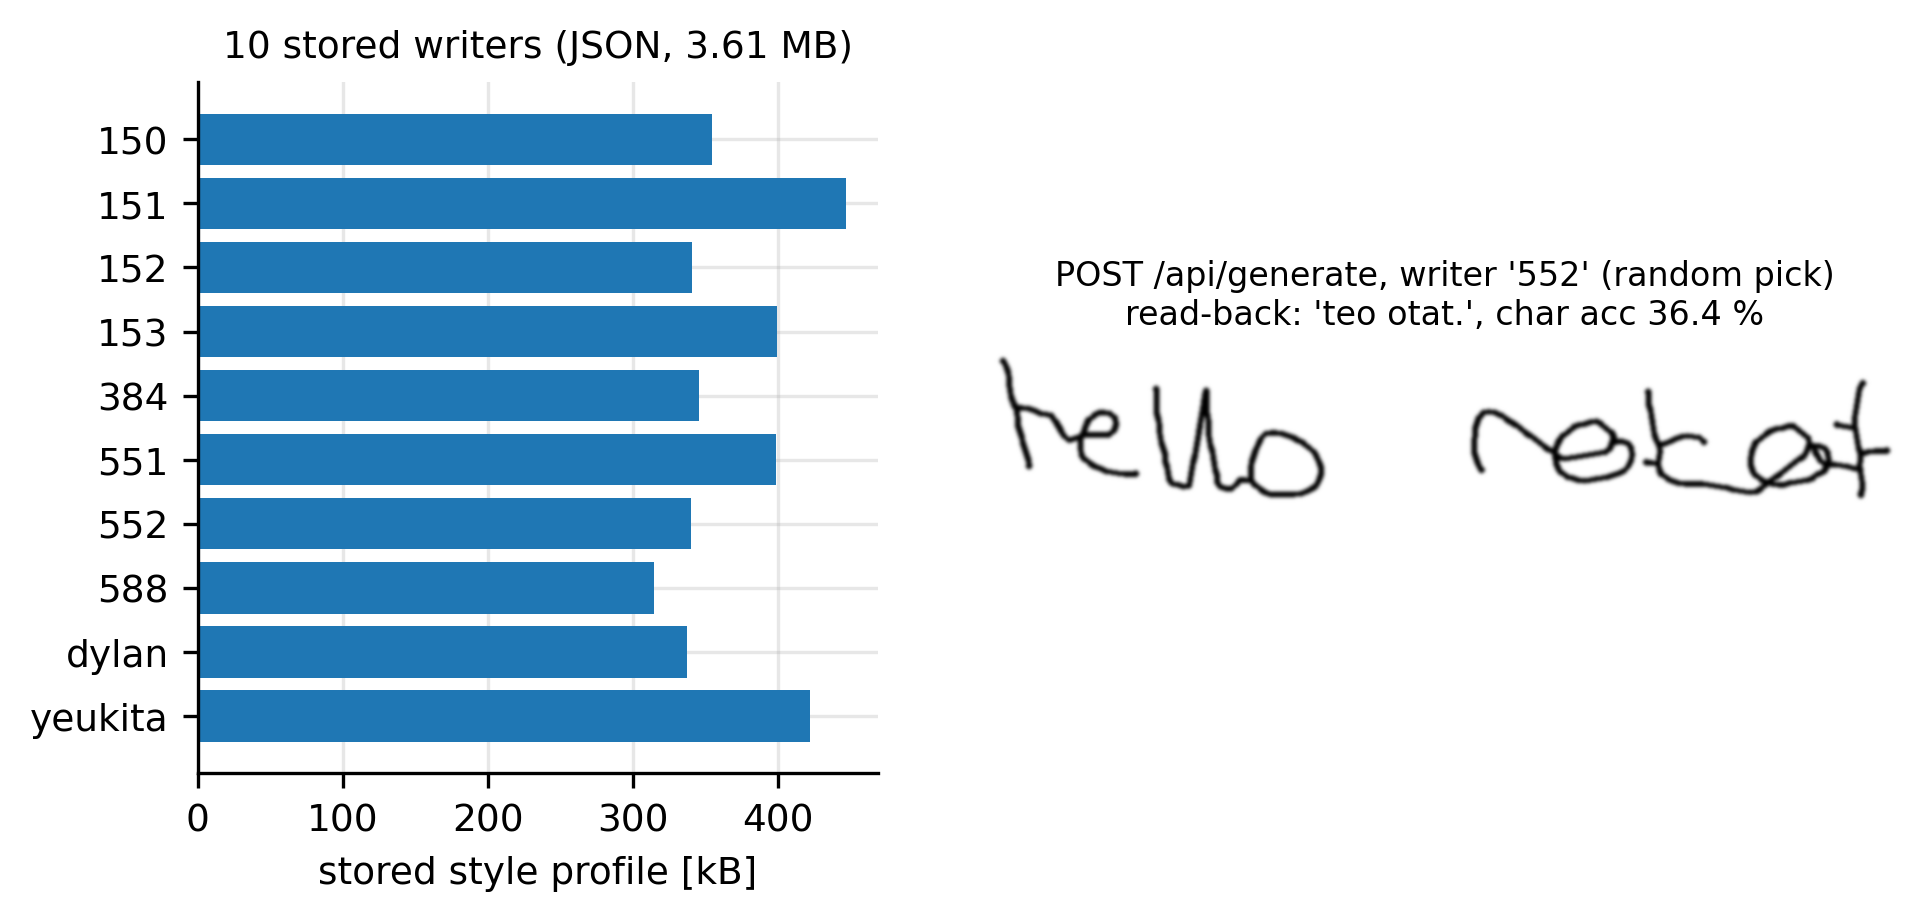
\includegraphics[width=0.82\linewidth]{Figures/qtp6_storage.png}
\caption{Storage of the writing styles. Each writer is held as a style profile and the server lists all thirteen through its author-list endpoint, against the ten required by R6.}
\label{fig:res-storage}
\end{figure}

        \QualificationSection{Observations}

            The list contained thirteen entries against a requirement of ten.
            The endpoint answered in 70~ms, so enumerating the stored styles is not a bottleneck for the user interface.
            The two personal writers are stored in the same format as the eleven database writers, so the storage mechanism does not distinguish between a writer whose pages were scanned and one whose pages were photographed.

        \QualificationSection{Statistical analysis}

            This is a count against a threshold and a pass or fail test; no statistical analysis is appropriate.
            The figure of thirteen is exact, not a sample estimate.
            Persistence follows from the profiles being files rather than in-memory state, and is observed each time the server starts and re-lists them; a power-cycle test of the board was not performed because the board was not deployed.


%%%%%%%%%%%%%%%%%%%%%%%%%%%%%%%%%%%%%%%%%%%%%%%%%%%%%%%%%%%%%%%%%%%%%%%%%%%%%%%%%

\subsubsection*{Field condition checks (FC1 and FC2)}
\label{sec:res-fc}

Neither field condition was measured.
\textbf{FC1:} a lux meter at the page plane records five points (centre and corners of an A4 page); the condition is met if all lie between 400 and 1000~lux, and qualification test 2 is repeated on the same pages at about 200, 700 and 1200~lux.
Illuminance: \nym{}; the flat-field correction and local thresholding should limit degradation within the range, with larger degradation below 400~lux.
\textbf{FC2:} a spirit level or inclinometer on both axes (tilt below $0.5^\circ$) and a logging accelerometer on the frame during a standard job, with the repeat error of qualification test 5 at rest and with a lightly tapped bench.
Tilt and vibration: \nym{}.

